\documentclass{beamer}

% Citations
\usepackage[style=apa, backend=biber, natbib]{biblatex}
\addbibresource{references.bib}

% Figures
\usepackage{graphicx}

% Links
\usepackage{hyperref}


% Title page components
\title{Extension of Gauchat (2012)---Politicization of Science in the Public Sphere: A Study of Public Trust in the United States, 1974 to 2021 [Draft]}
\subtitle{Presentation of Figures}
\author{Clemens Stefan Heithecker}
\institute{Tilburg University}


% Change primary color to black
\definecolor{beamer@blendedblue}{rgb}{0, 0, 0}

% Custom section page
\defbeamertemplate{section page}{custom}[1][]{%
  \begin{centering}
    {\usebeamerfont{section name}\usebeamercolor[fg]{section name}#1}
    \vskip1em\par
    \begin{beamercolorbox}[sep=12pt,center]{part title}
      \usebeamerfont{section title}\insertsection\par
    \end{beamercolorbox}
  \end{centering}
}

% Custom subsection page
\defbeamertemplate{subsection page}{custom}[1][]{%
  \begin{centering}
    {\usebeamerfont{subsection name}\usebeamercolor[fg]{subsection name}#1}
    \vskip1em\par
    \begin{beamercolorbox}[sep=8pt,center,#1]{part title}
      \usebeamerfont{subsection title}\insertsubsection\par
    \end{beamercolorbox}
  \end{centering}
}

% Select custom section and subsection pages
\setbeamertemplate{section page}[custom]
\setbeamertemplate{subsection page}[custom]

% Remove icons in bibliography
\setbeamertemplate{bibliography item}{}

% Automatically generate a section title frame

\newif\ifSectionTitlePage
\newcommand*\SectionTitlePagedefault{\SectionTitlePagefalse}

\newcommand\AllSectionsWithTitlePage{%
  \SectionTitlePagetrue
  \renewcommand*\SectionTitlePagedefault{\SectionTitlePagetrue}%
}
\newcommand\AllSectionsWithoutTitlePage{%
  \SectionTitlePagefalse
  \renewcommand*\SectionTitlePagedefault{\SectionTitlePagefalse}%
}
\newcommand\NextSectionWithTitlePage{\SectionTitlePagetrue}
\newcommand\NextSectionWithoutTitlePage{\SectionTitlePagefalse}

\AtBeginSection[]{
	\ifSectionTitlePage
		\frame{\sectionpage}
	\fi
	\SectionTitlePagedefault
}

% Enable the title pages
\AllSectionsWithTitlePage


% Change the text color of the bibliography
\setbeamercolor{bibliography item}{fg=black}
\setbeamercolor{bibliography entry author}{fg=black}
\setbeamercolor{bibliography entry title}{fg=black}
\setbeamercolor{bibliography entry location}{fg=black}
\setbeamercolor{bibliography entry note}{fg=black}


\begin{document}

% Include references in the bibliography without in-text citing
\nocite{davern-2021}
\nocite{gauchat-2012}


\frame{\titlepage}

\frame{ \frametitle{Contents}	\tableofcontents }


\section{Missing Values}

\subsection{Missing Values Summary}

\begin{frame}{Missing Values Summary (1)}
\begin{figure}
	\centerline{
		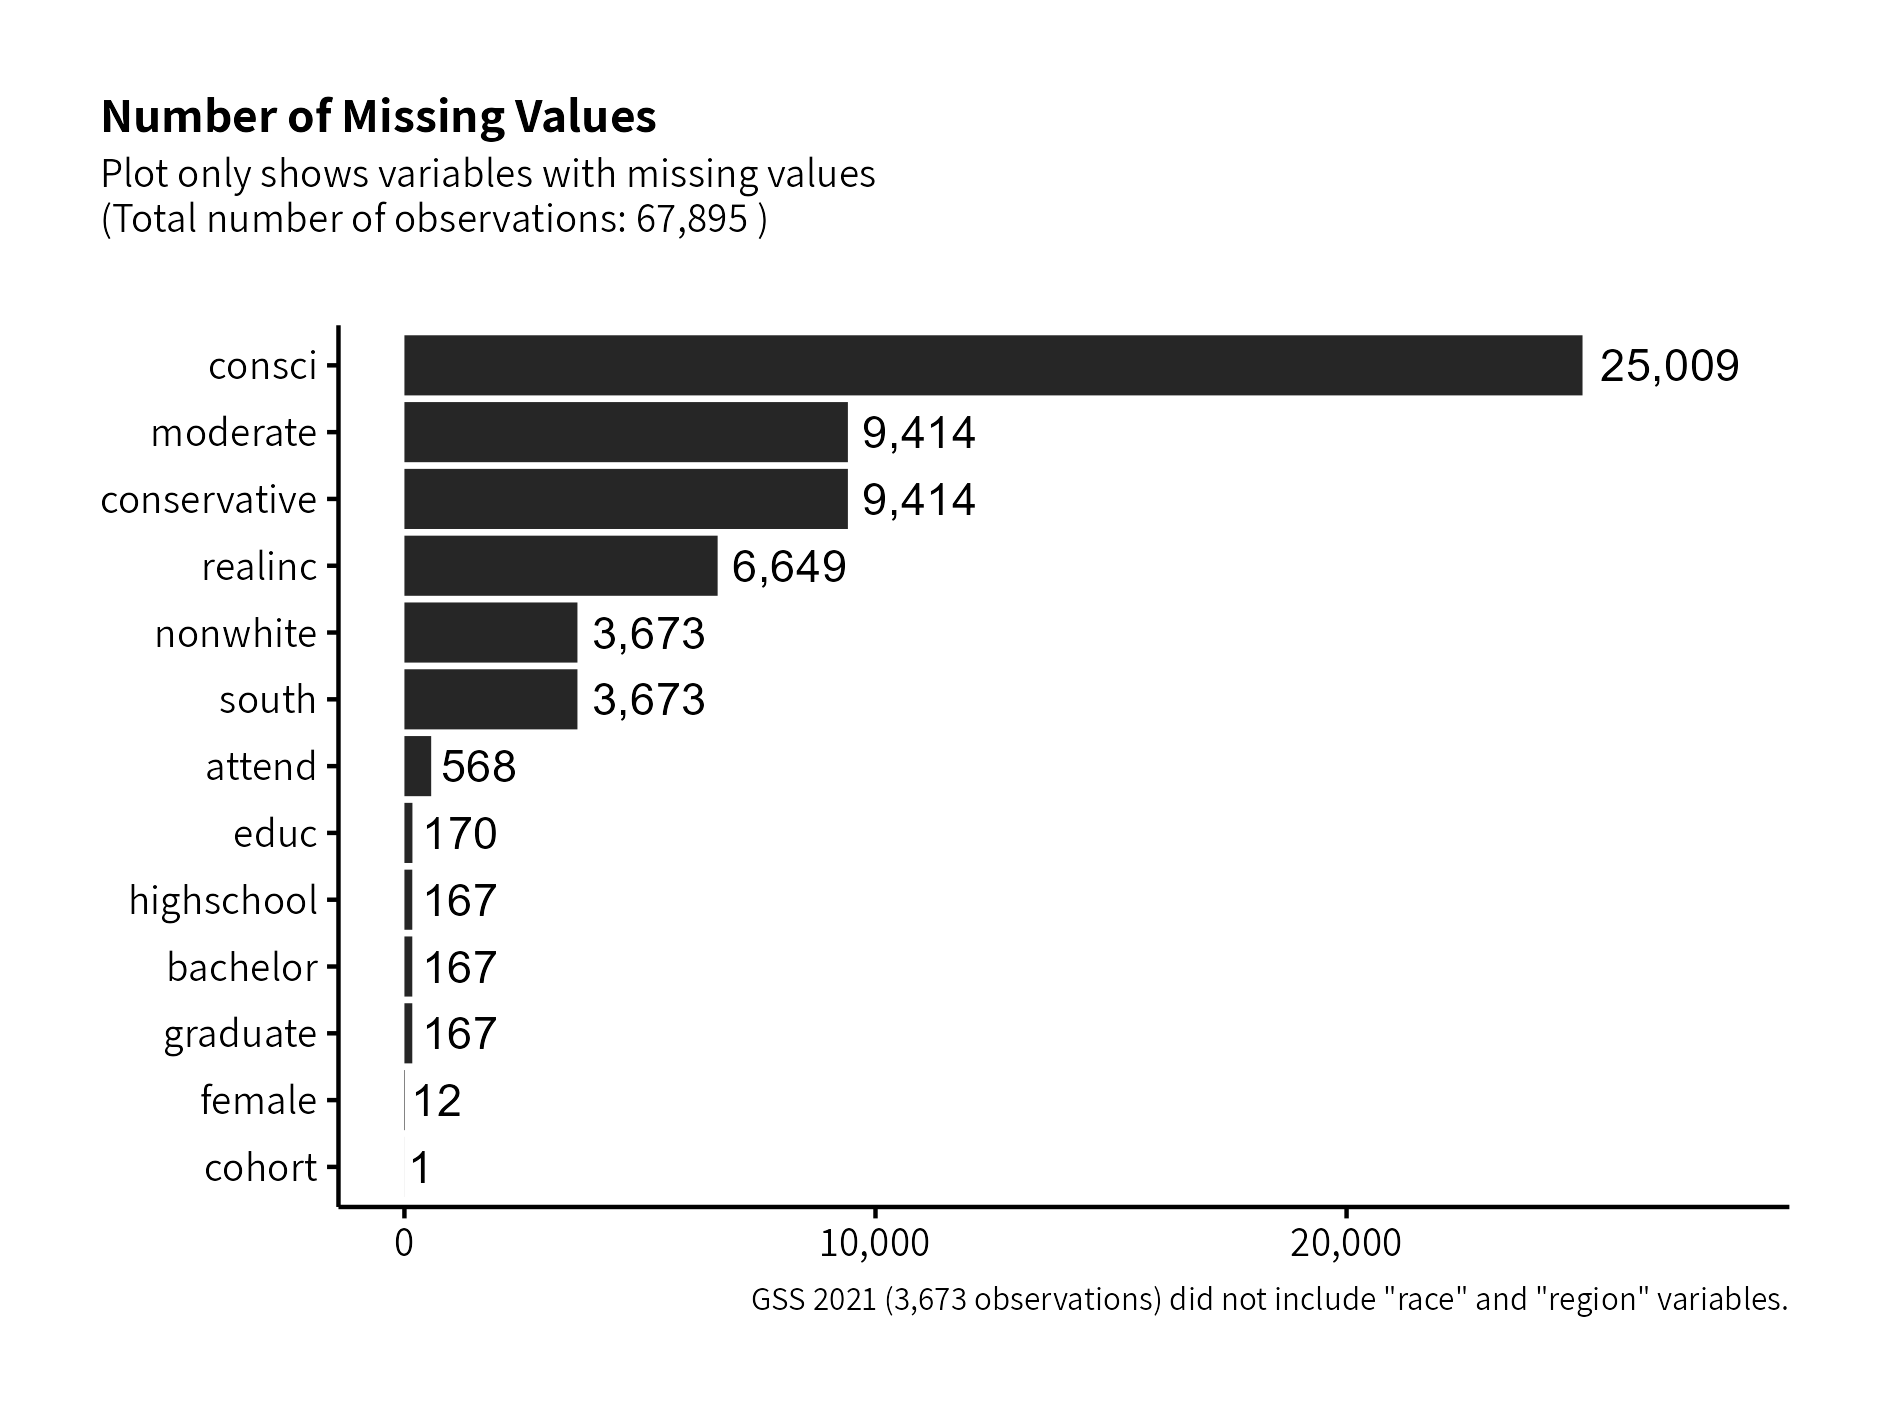
\includegraphics[width=0.8\paperwidth, keepaspectratio]{ {../figures/missing-values-count} }
	}
\end{figure}
\end{frame}

\begin{frame}{Missing Values Summary (2)}
\begin{figure}
	\centerline{
		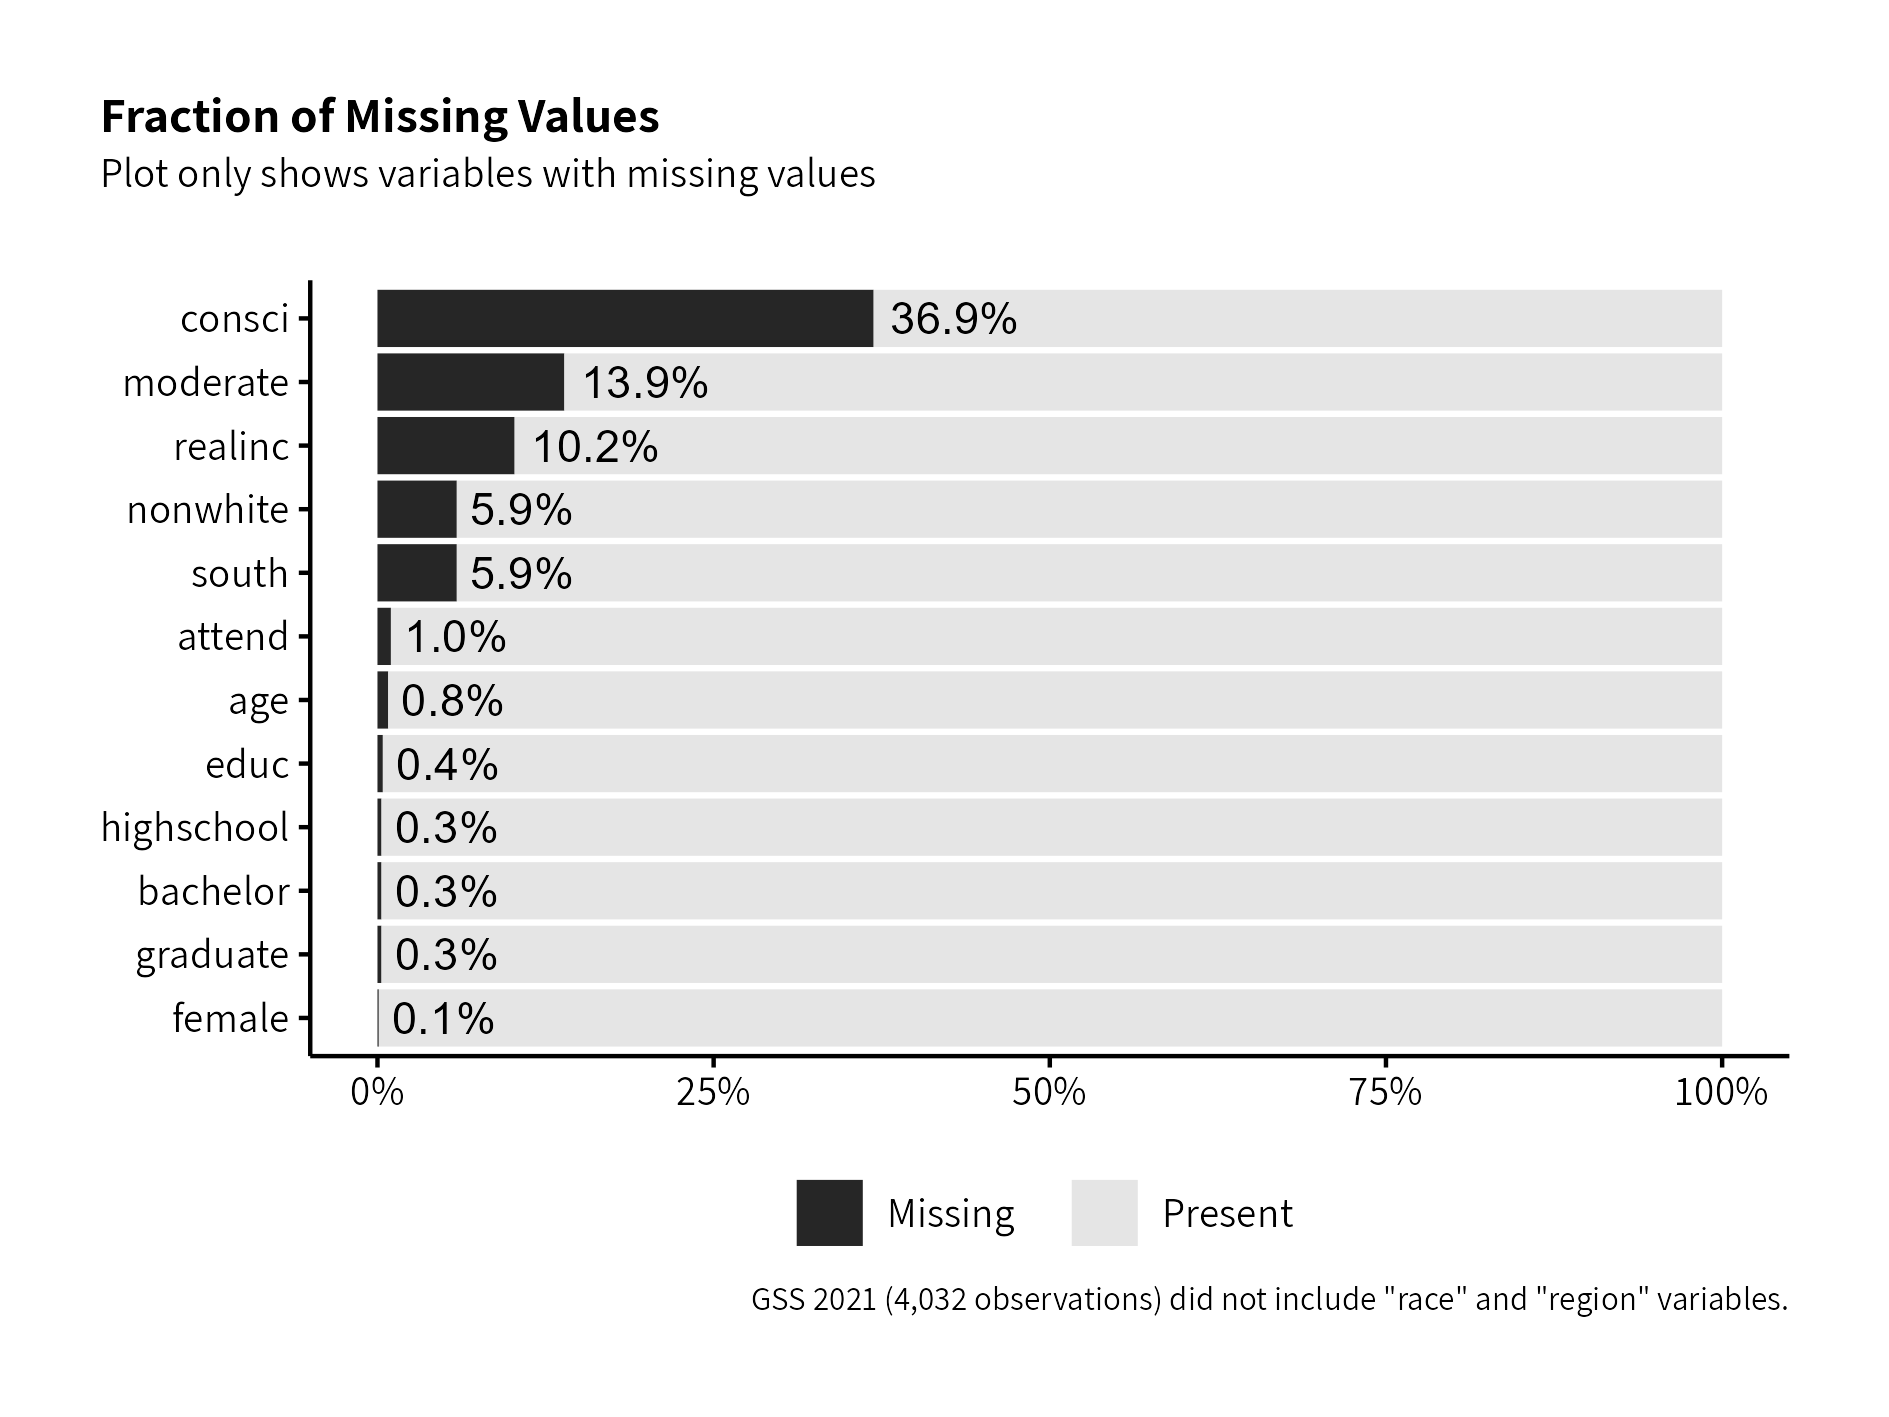
\includegraphics[width=0.8\paperwidth, keepaspectratio]{ {../figures/missing-values-fraction} }
	}
\end{figure}
\end{frame}


\subsection{Comparison of Data With(out) Missing Income Values}

\begin{frame}{Comparison of Data With(out) Missing Income Values}
\begin{figure}
	\centerline{
		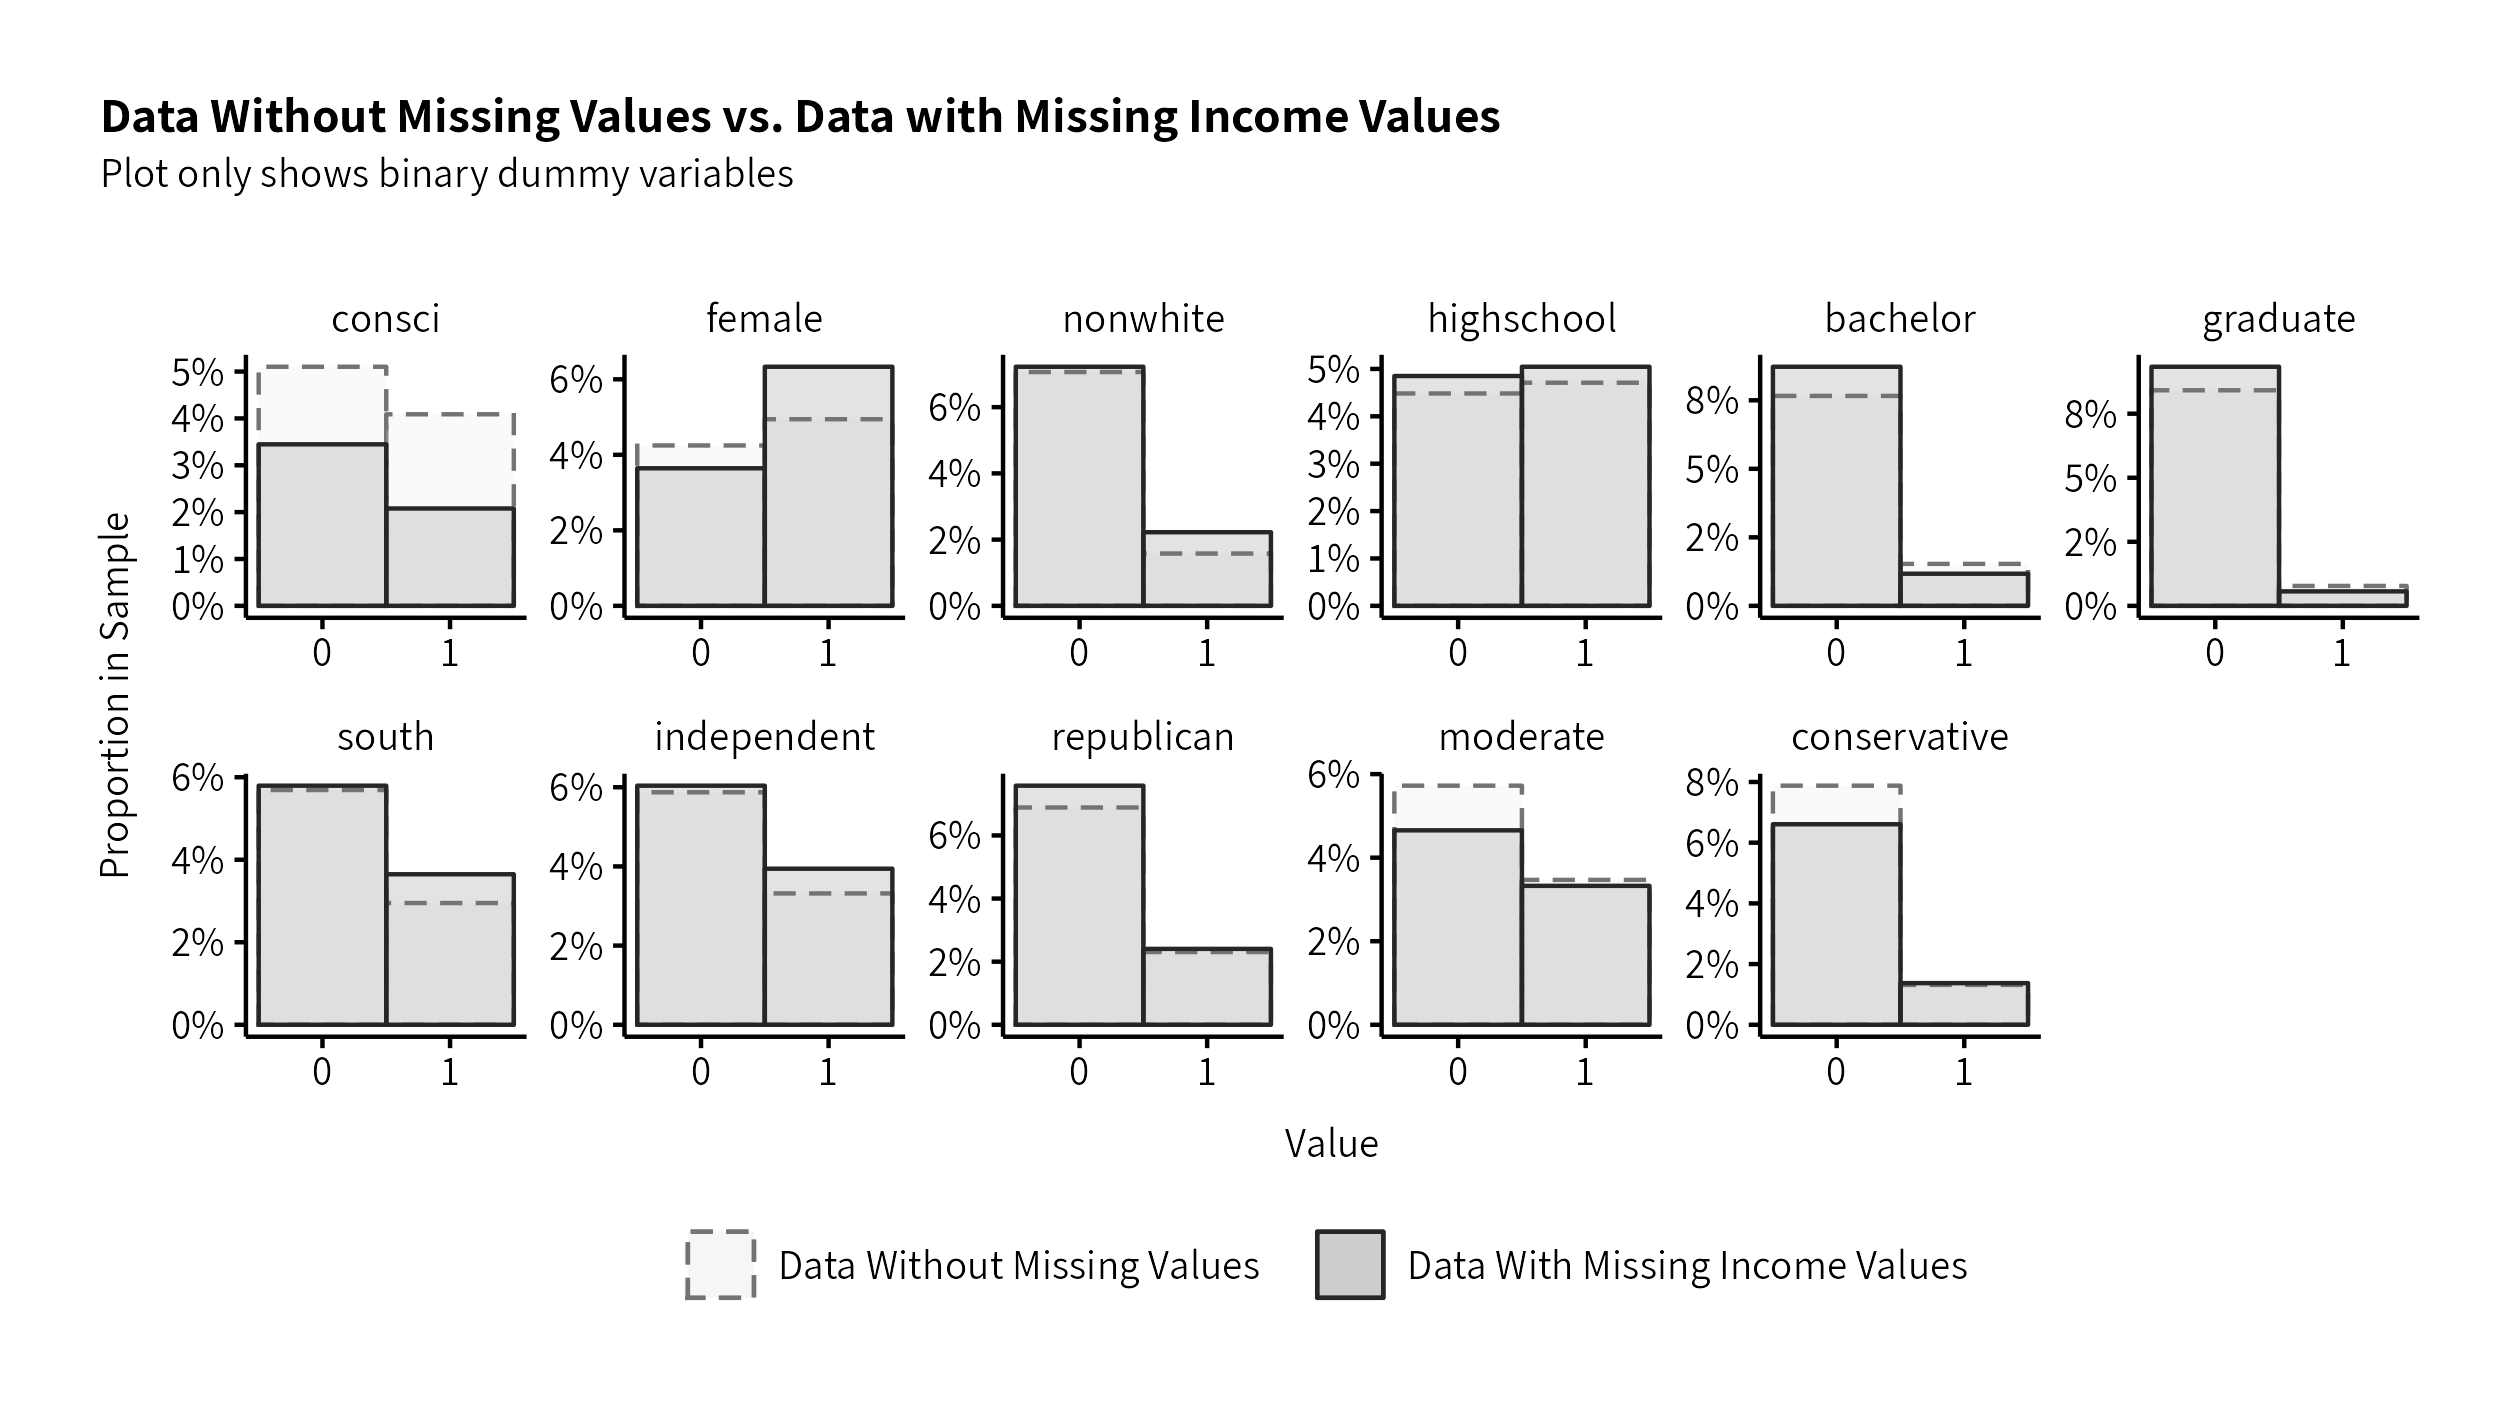
\includegraphics[width=0.8\paperwidth, keepaspectratio]{ {../figures/missing-values-distributions-wide} }
	}
\end{figure}
\end{frame}


\subsection{Missing Values by Year}

\begin{frame}{Missing Values by Year (1)}
\begin{figure}
	\centerline{
		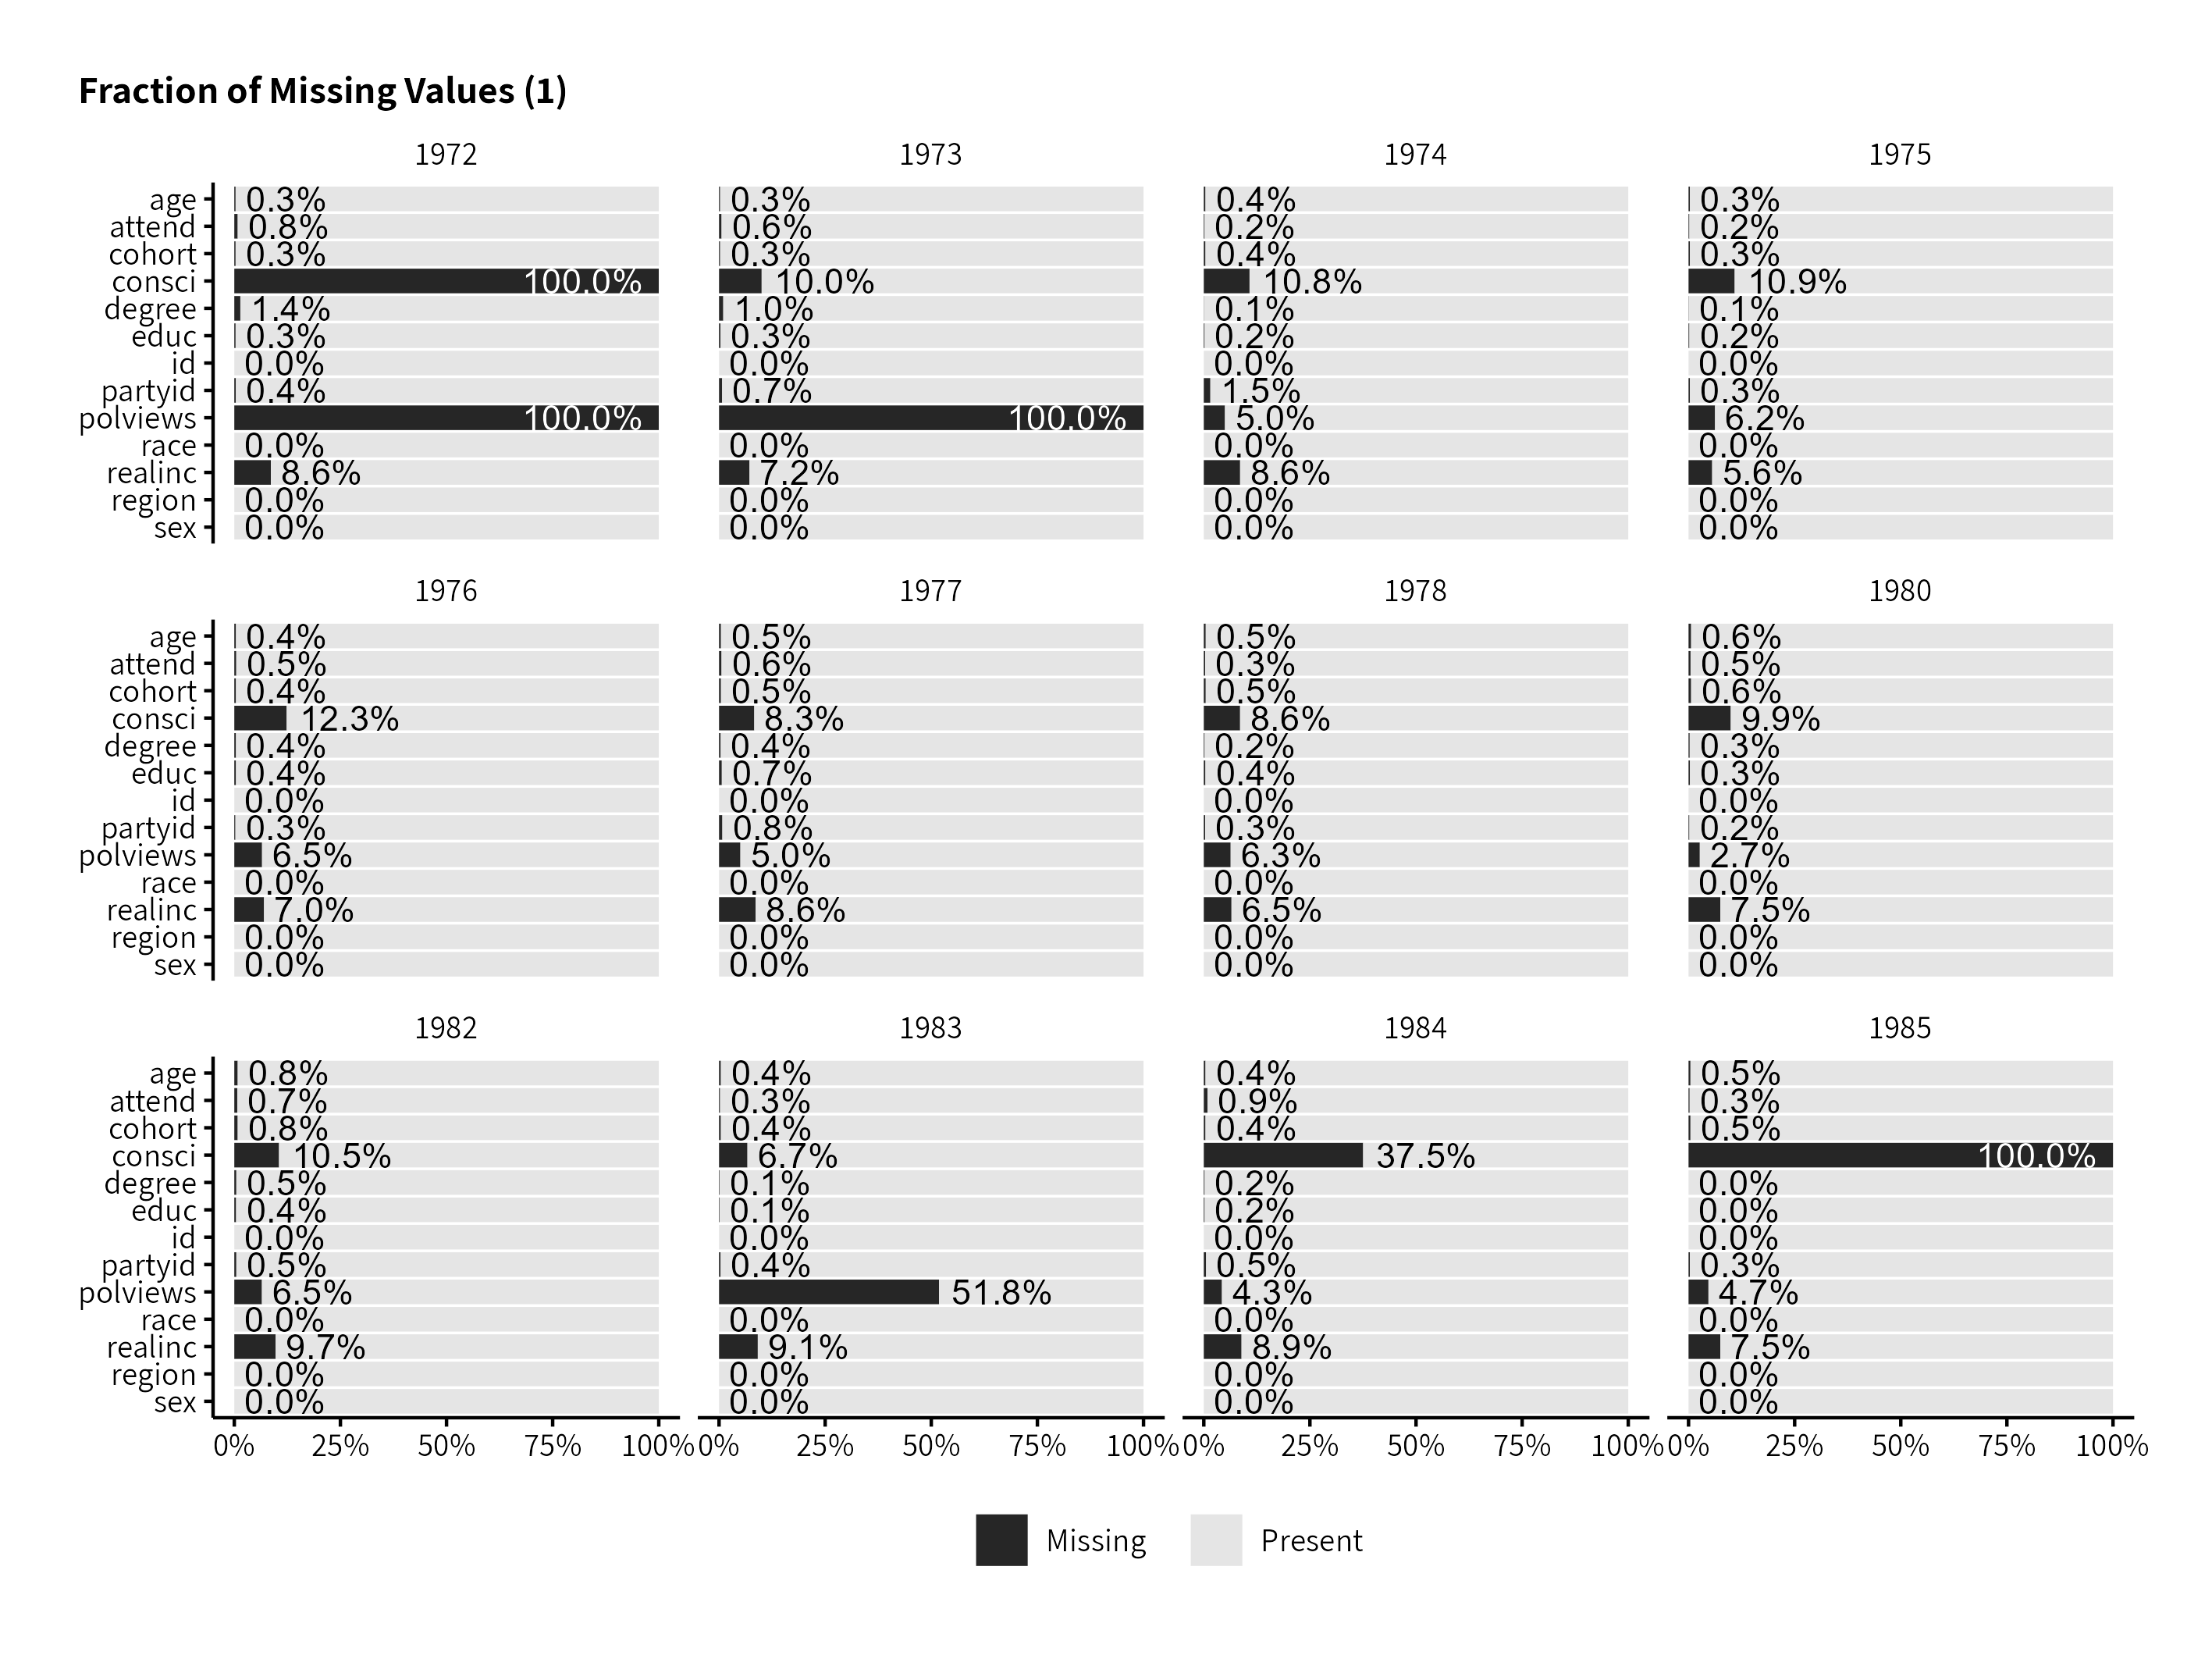
\includegraphics[width=0.8\paperwidth, keepaspectratio]{ {../figures/missing-values-variable-year-1} }
	}
\end{figure}
\end{frame}

\begin{frame}{Missing Values by Year (2)}
\begin{figure}
	\centerline{
		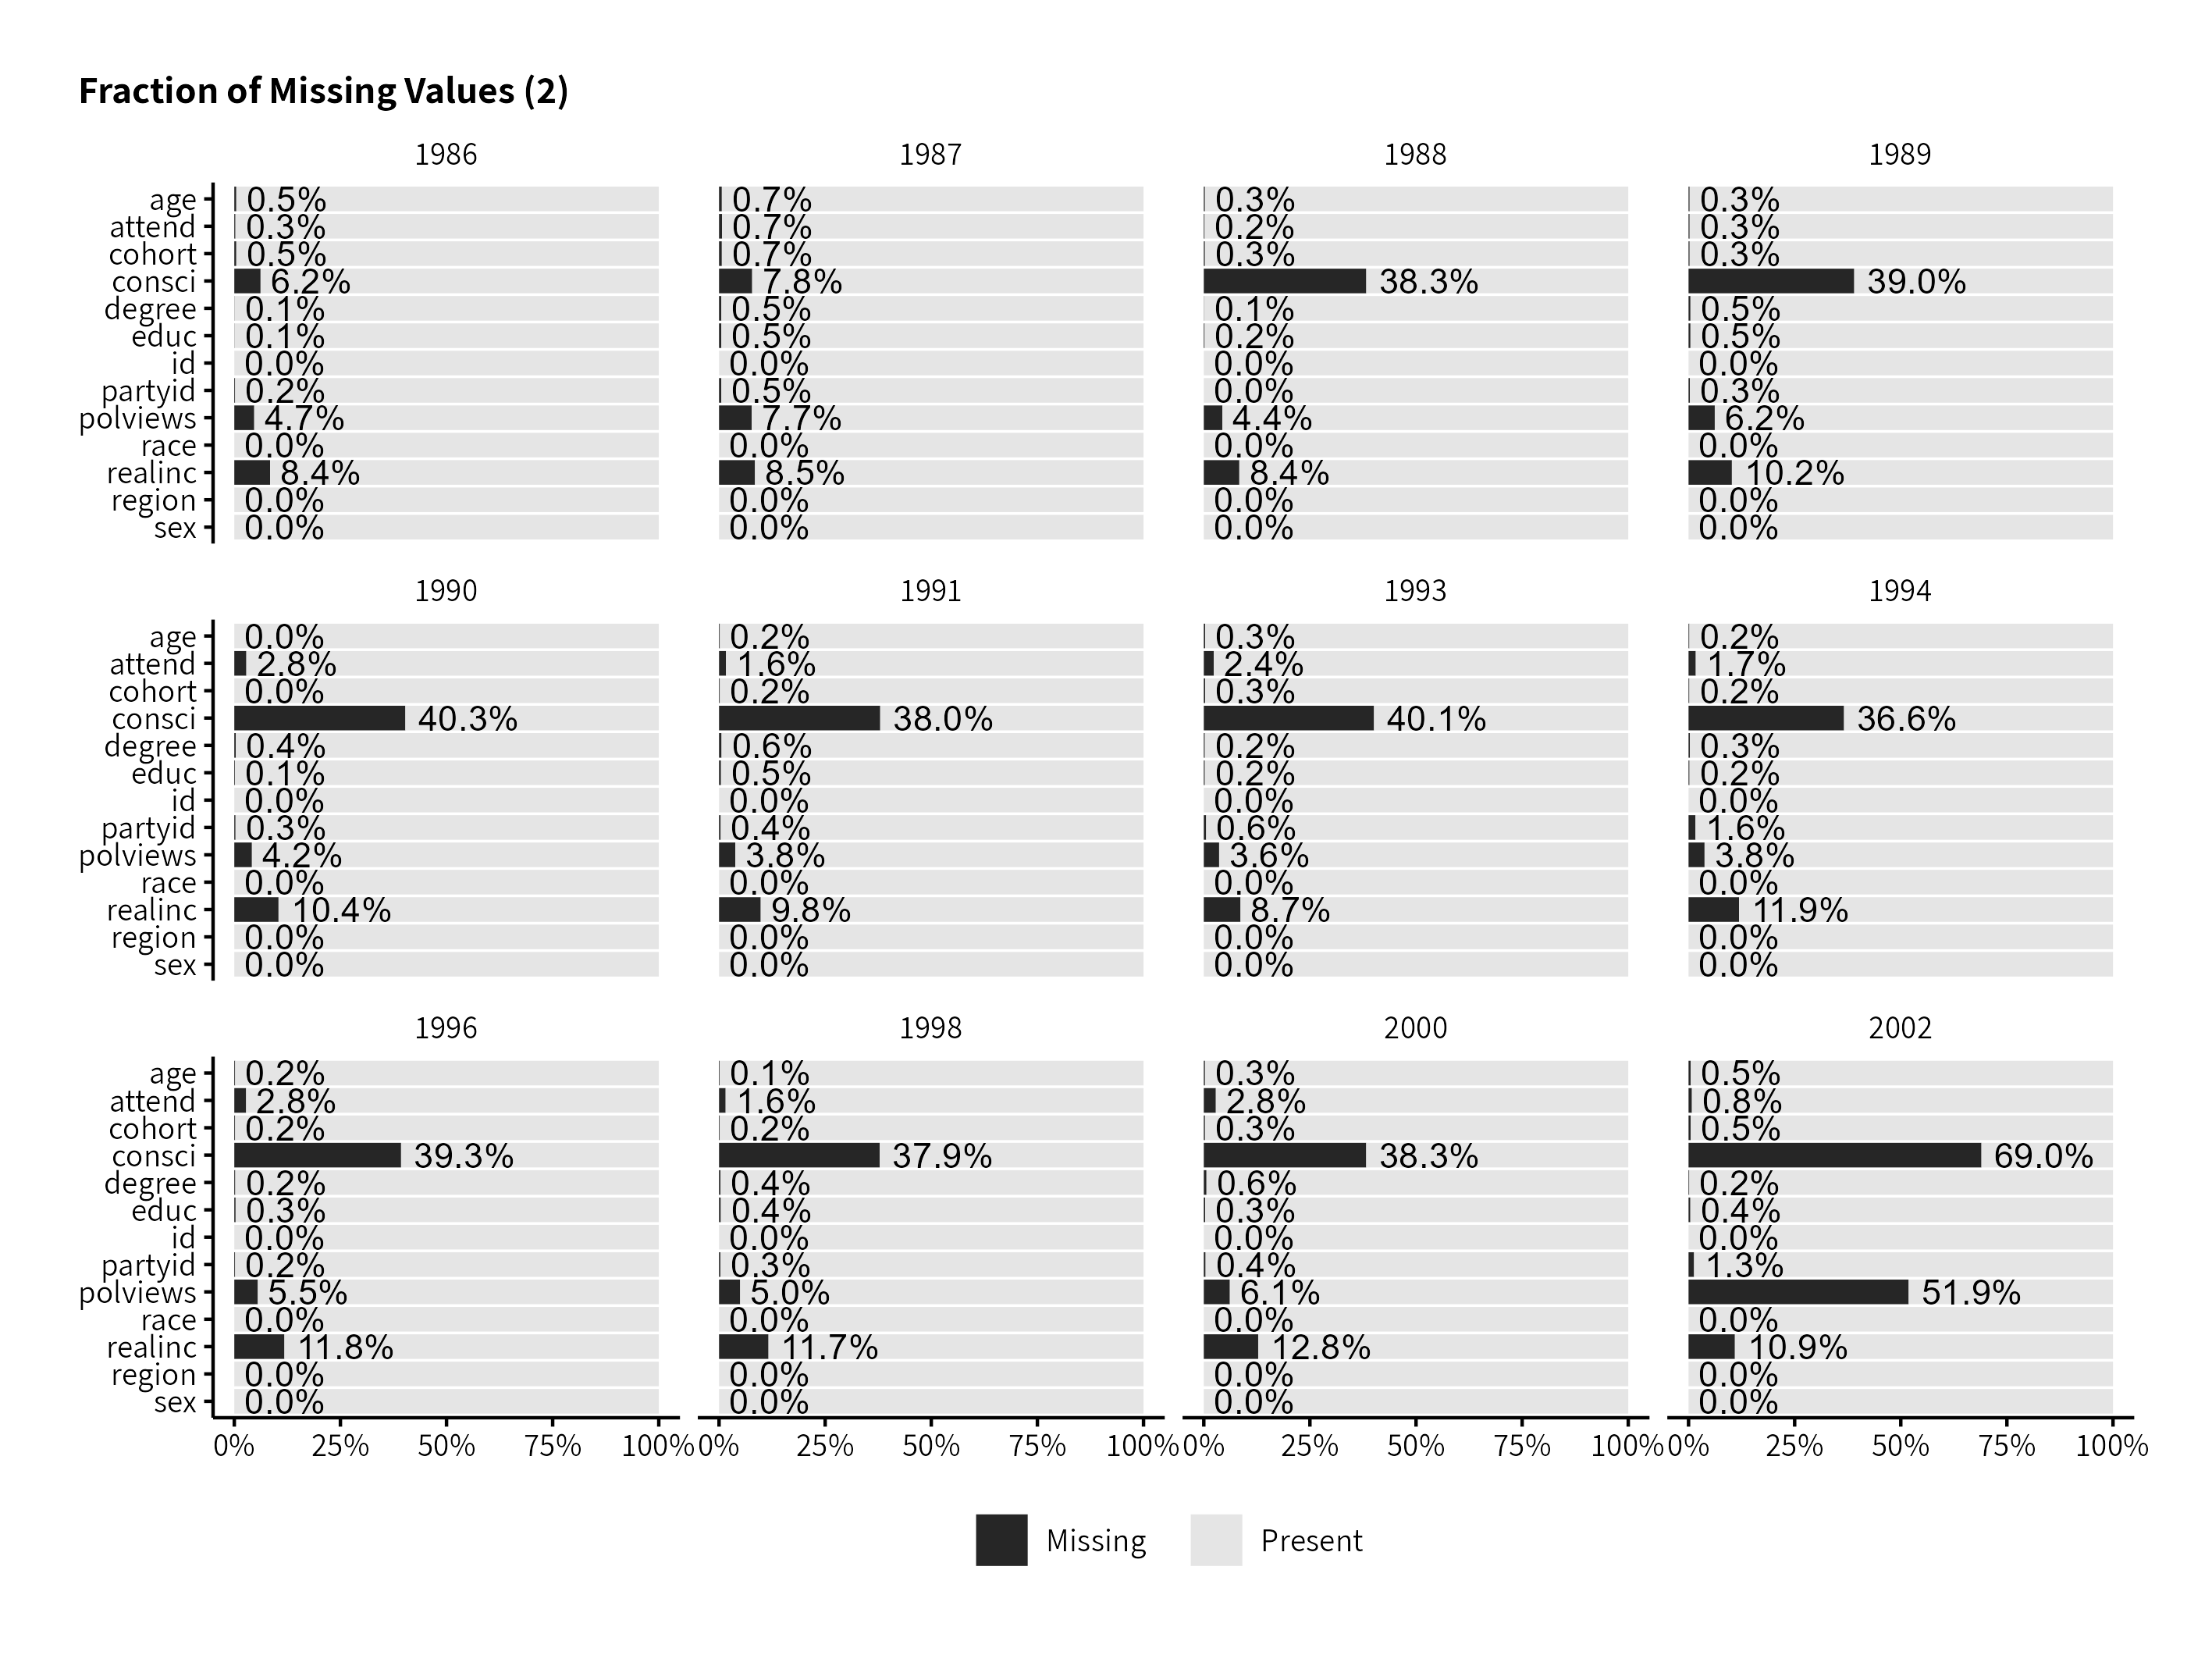
\includegraphics[width=0.8\paperwidth, keepaspectratio]{ {../figures/missing-values-variable-year-2} }
	}
\end{figure}
\end{frame}

\begin{frame}{Missing Values by Year (3)}
\begin{figure}
	\centerline{
		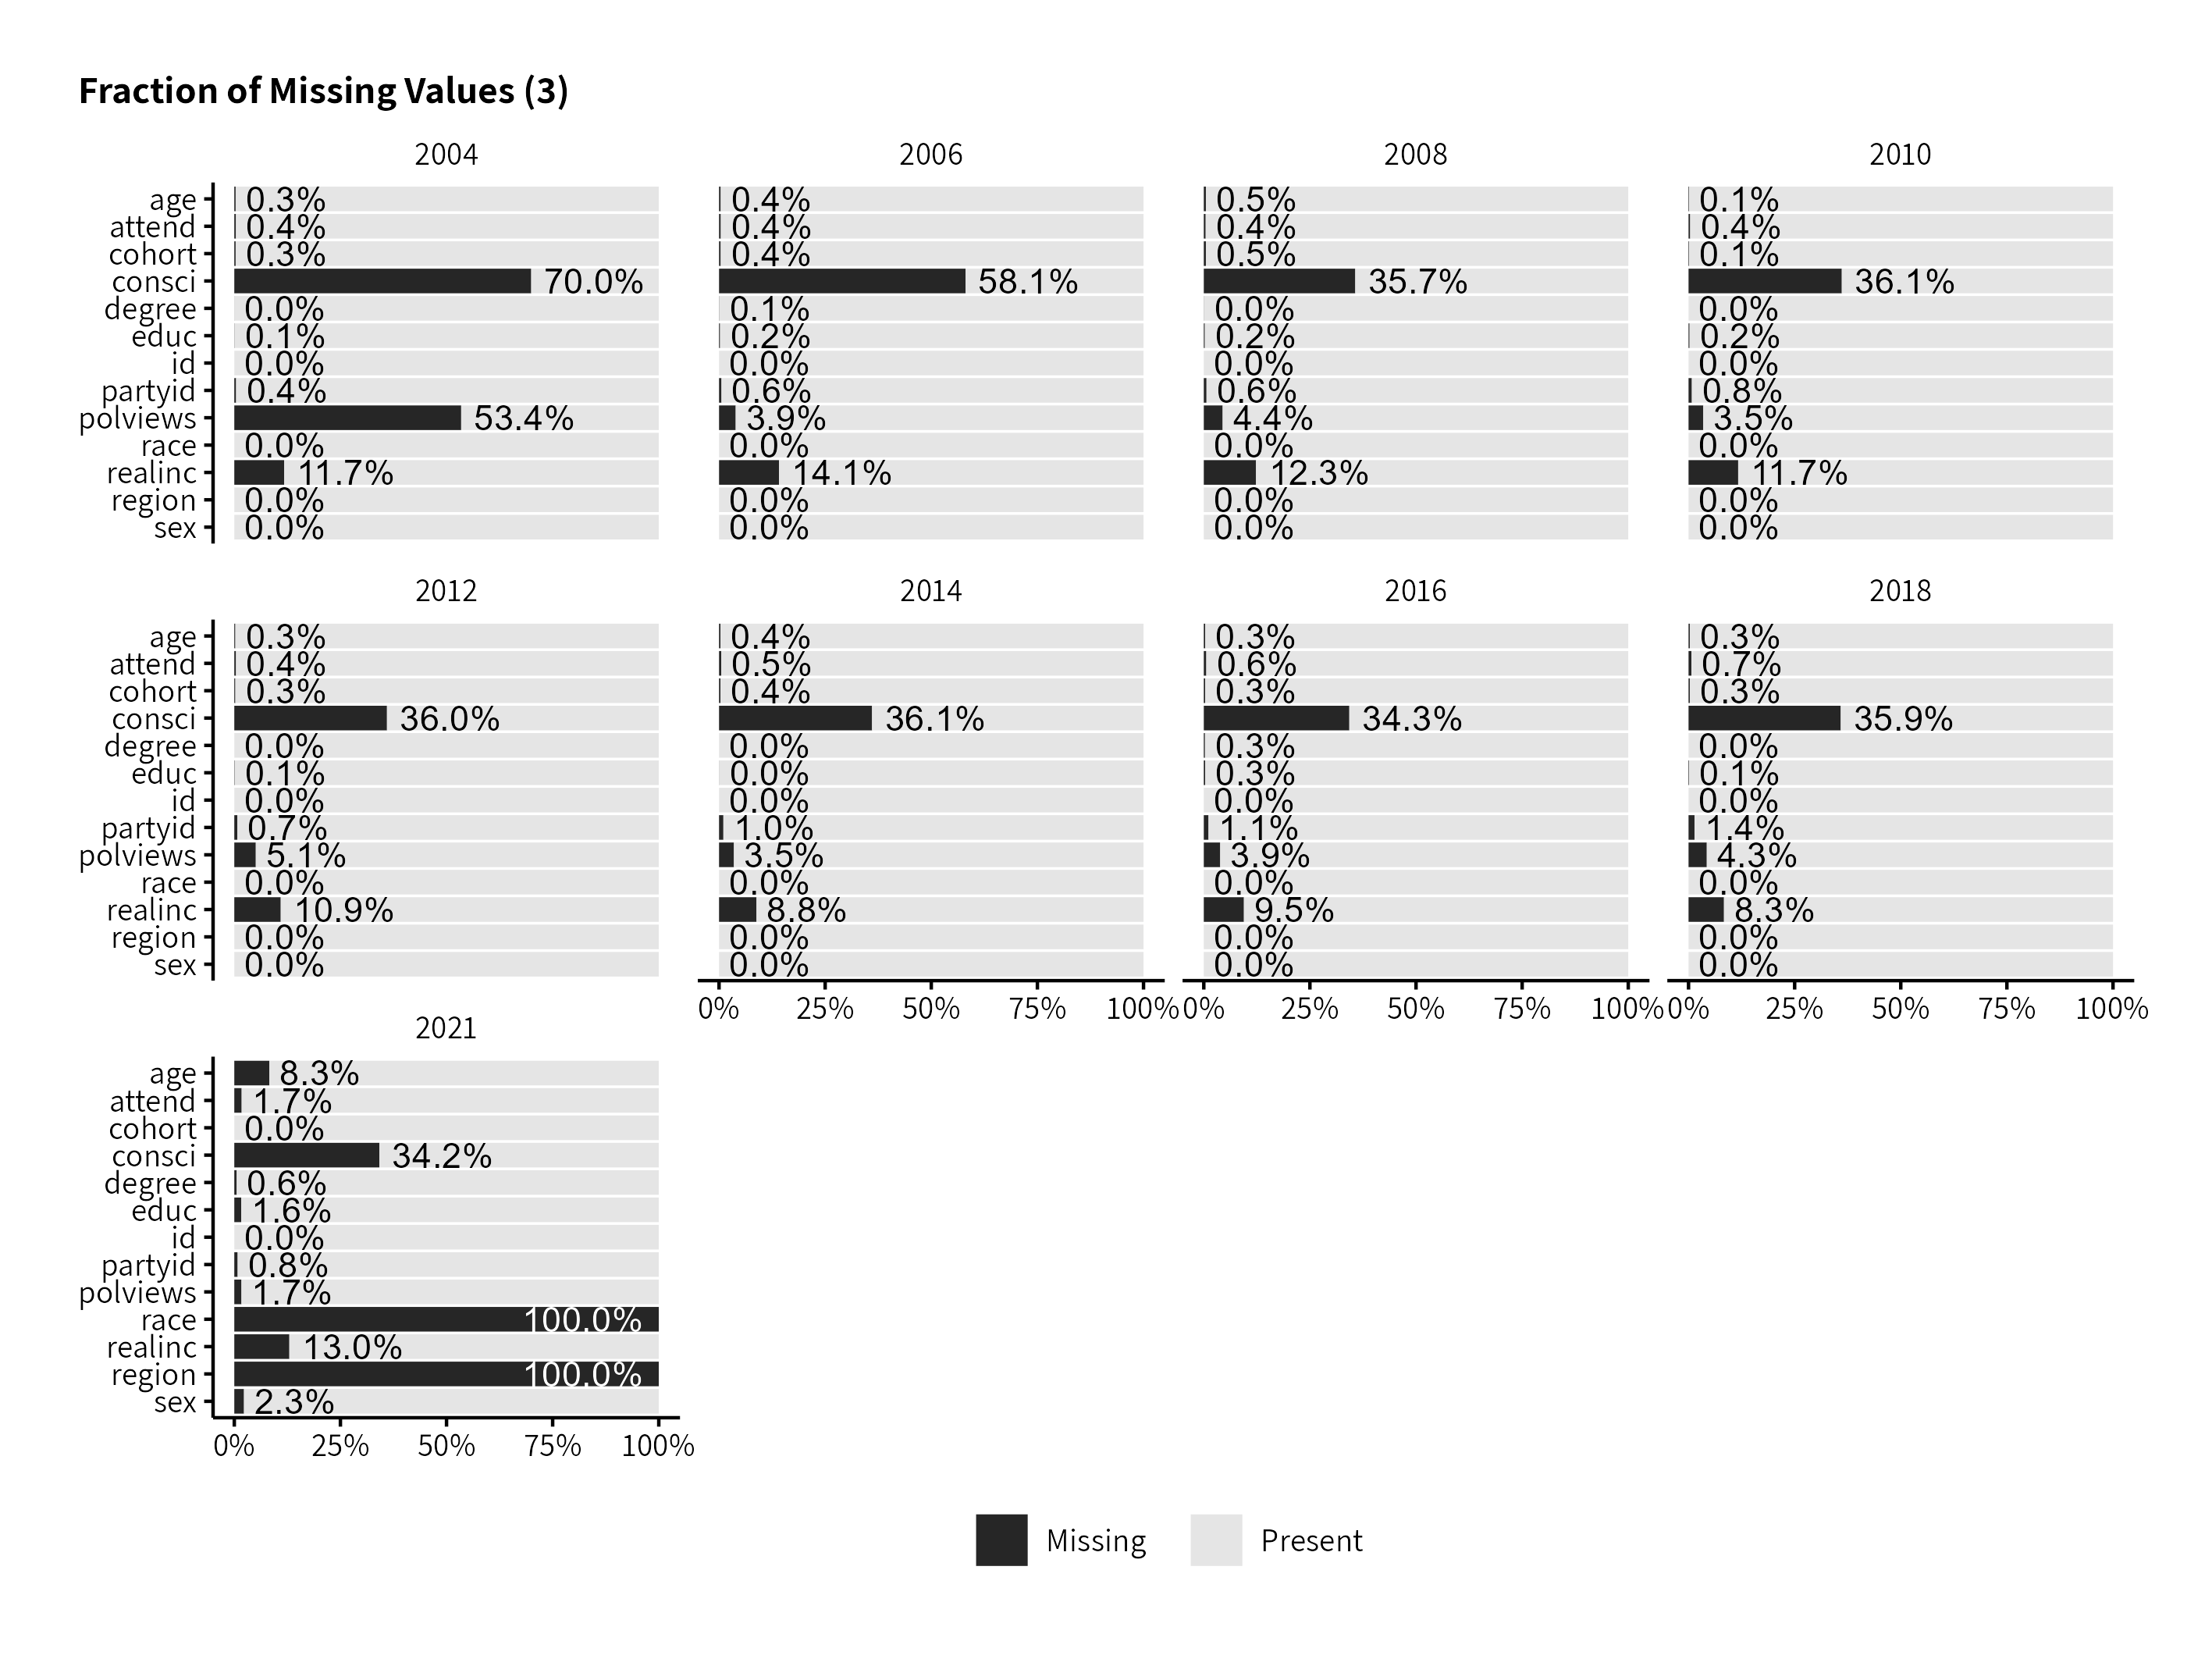
\includegraphics[width=0.8\paperwidth, keepaspectratio]{ {../figures/missing-values-variable-year-3} }
	}
\end{figure}
\end{frame}


\section{Aggregate Statistics}

\subsection{Confidence in Science by Political Ideology Over Time}

\begin{frame}
\frametitle{Confidence in Science by Political Ideology Over Time (1)}
\framesubtitle{Cleaned Sample}
\begin{figure}
	\centerline{
		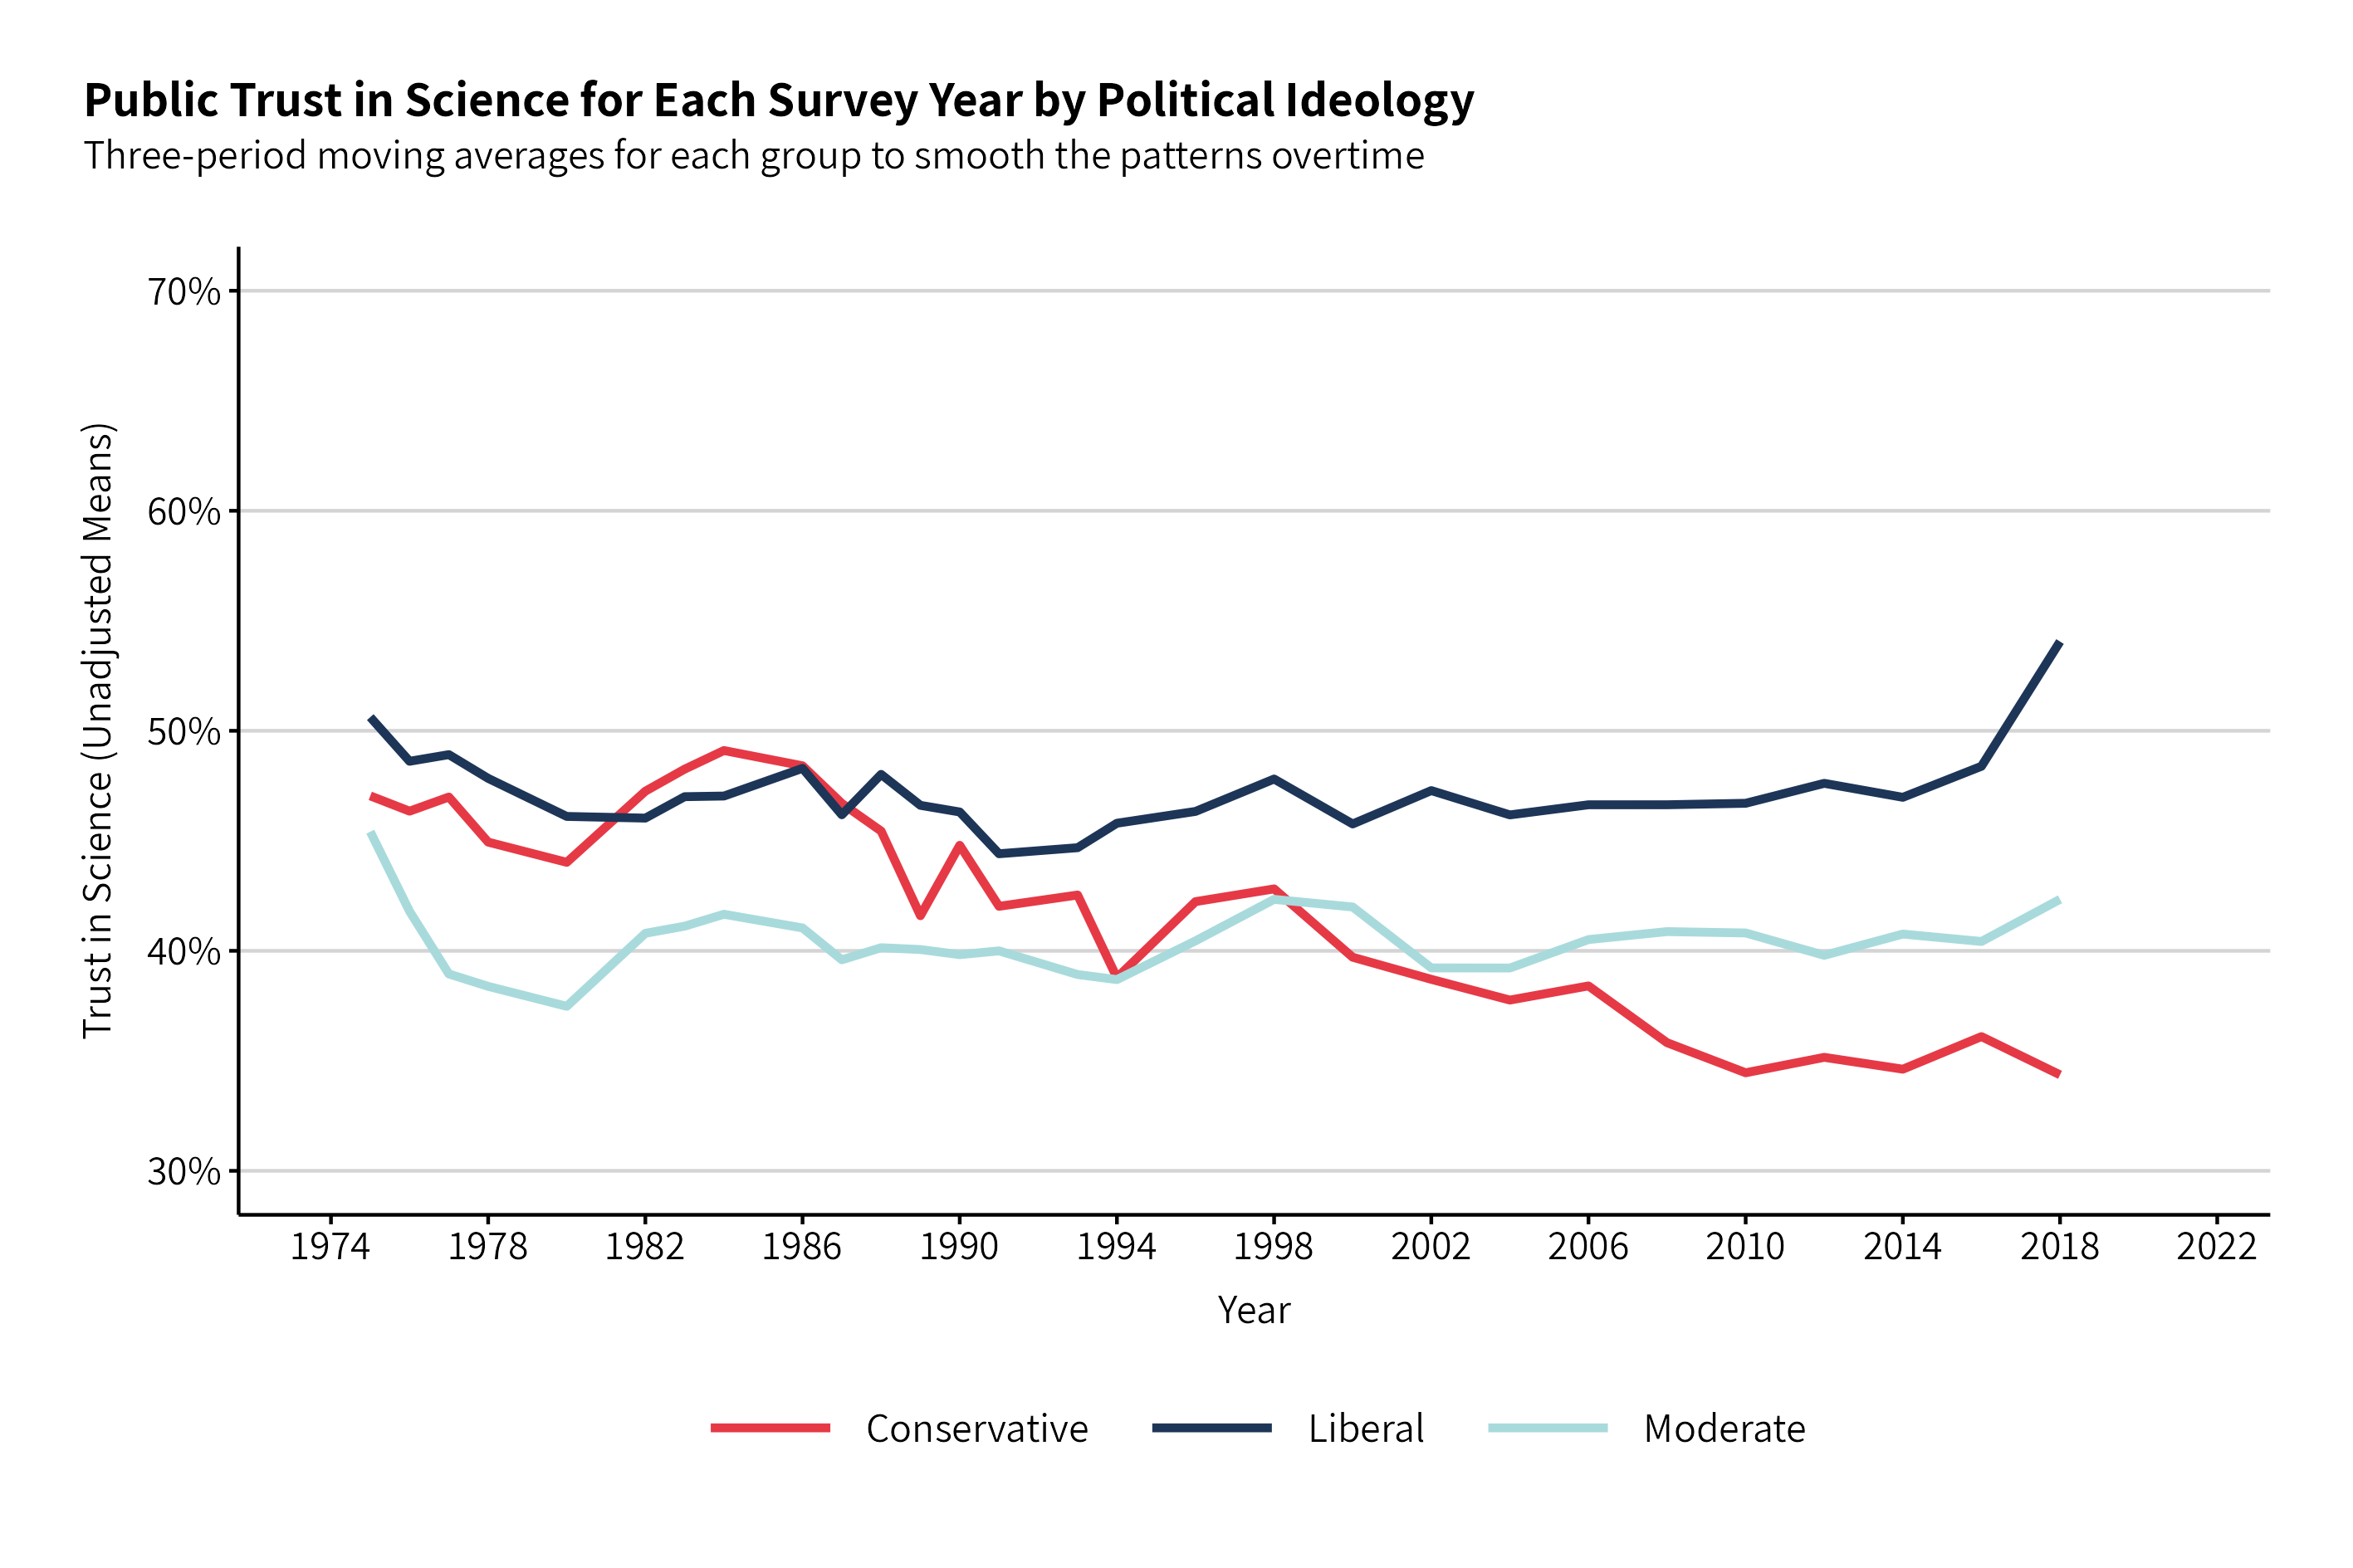
\includegraphics[width=0.75\paperwidth, keepaspectratio]{ {../figures/consci-by-polviews} }
	}
\end{figure}
\end{frame}

\begin{frame}
\frametitle{Confidence in Science by Political Ideology Over Time (2)}
\framesubtitle{Pre-Cleaned Sample Including Missing Values}
\begin{figure}
	\centerline{
		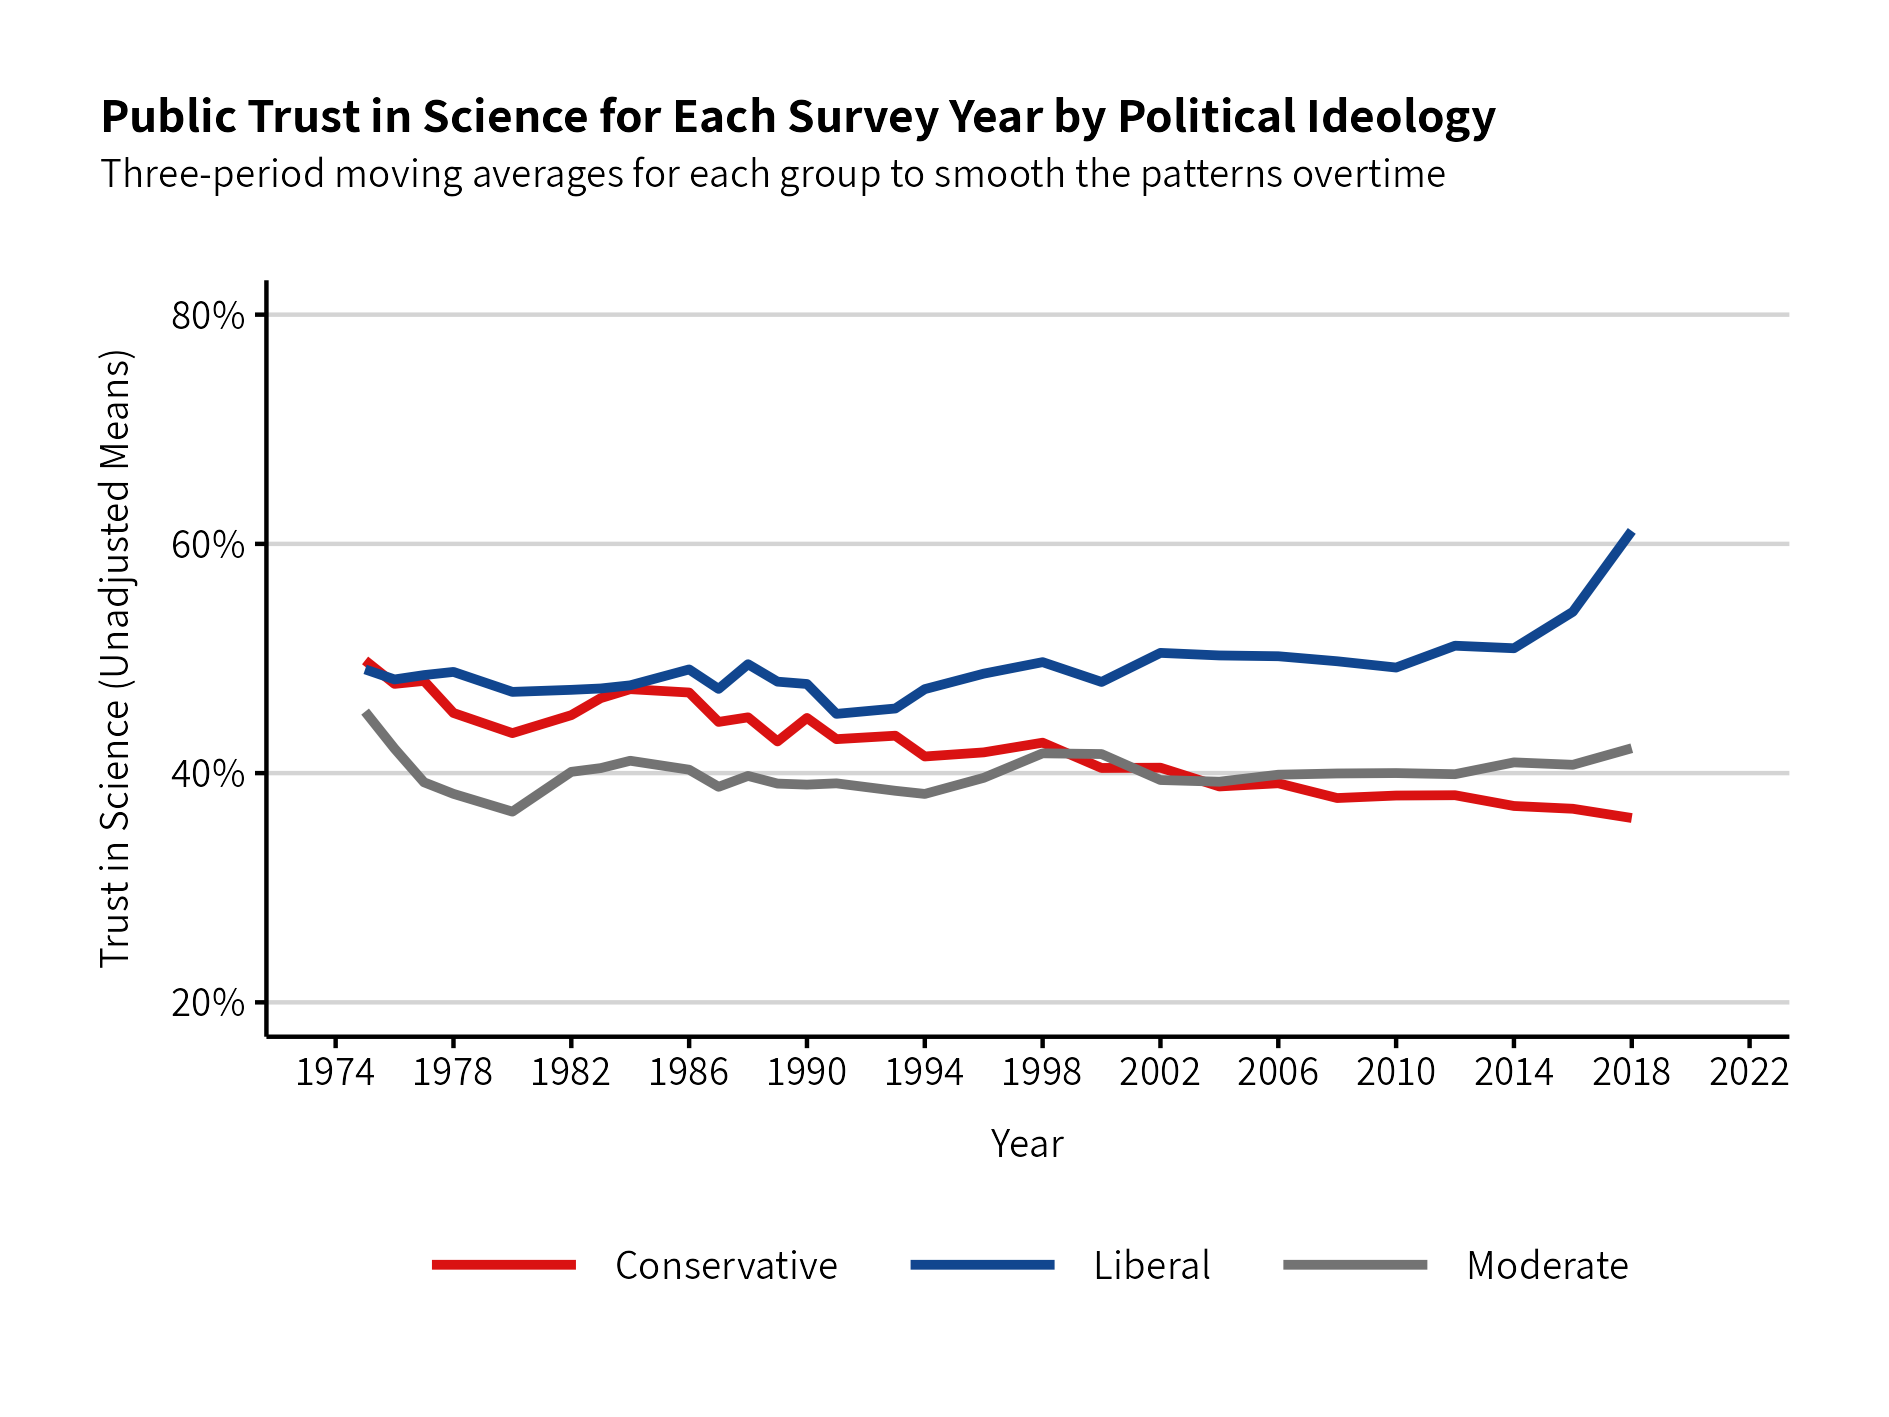
\includegraphics[width=0.75\paperwidth, keepaspectratio]{ {../figures/consci-by-polviews-with-na} }
	}
\end{figure}
\end{frame}


\section{Predictive Analysis}

\subsection{Predicted Trust in Science, \textit{Excluding} 2021}

\begin{frame}{Predicted Trust in Science, \textit{Excluding} 2021 (1)}
\begin{figure}
	\centerline{
		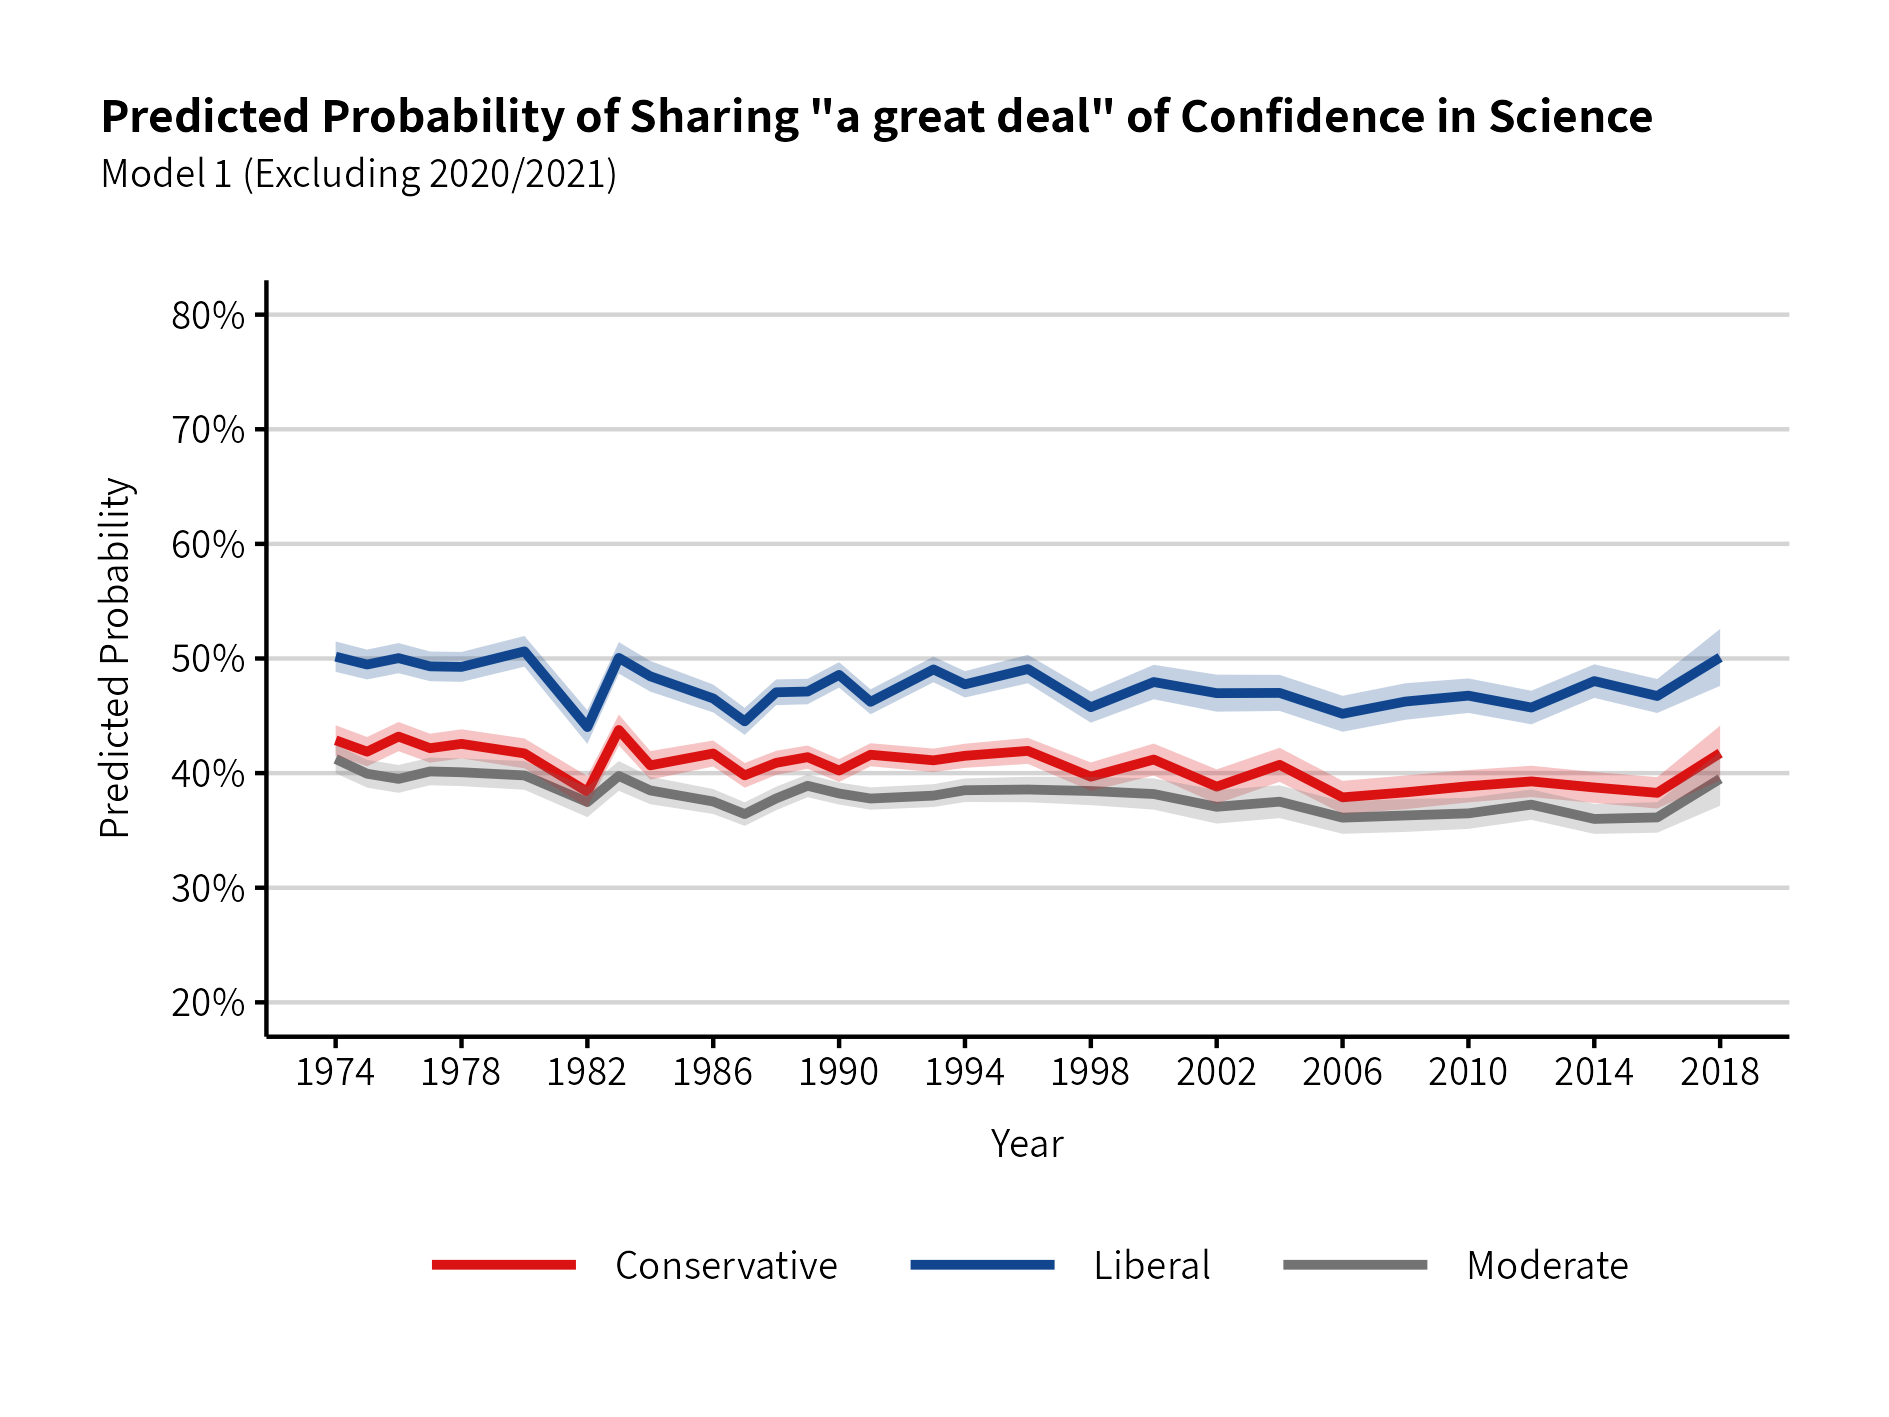
\includegraphics[width=0.8\paperwidth, keepaspectratio]{ {../figures/predict-polview-year-model-1} }
	}
\end{figure}
\end{frame}

\begin{frame}{Predicted Trust in Science, \textit{Excluding} 2021 (2)}
\begin{figure}
	\centerline{
		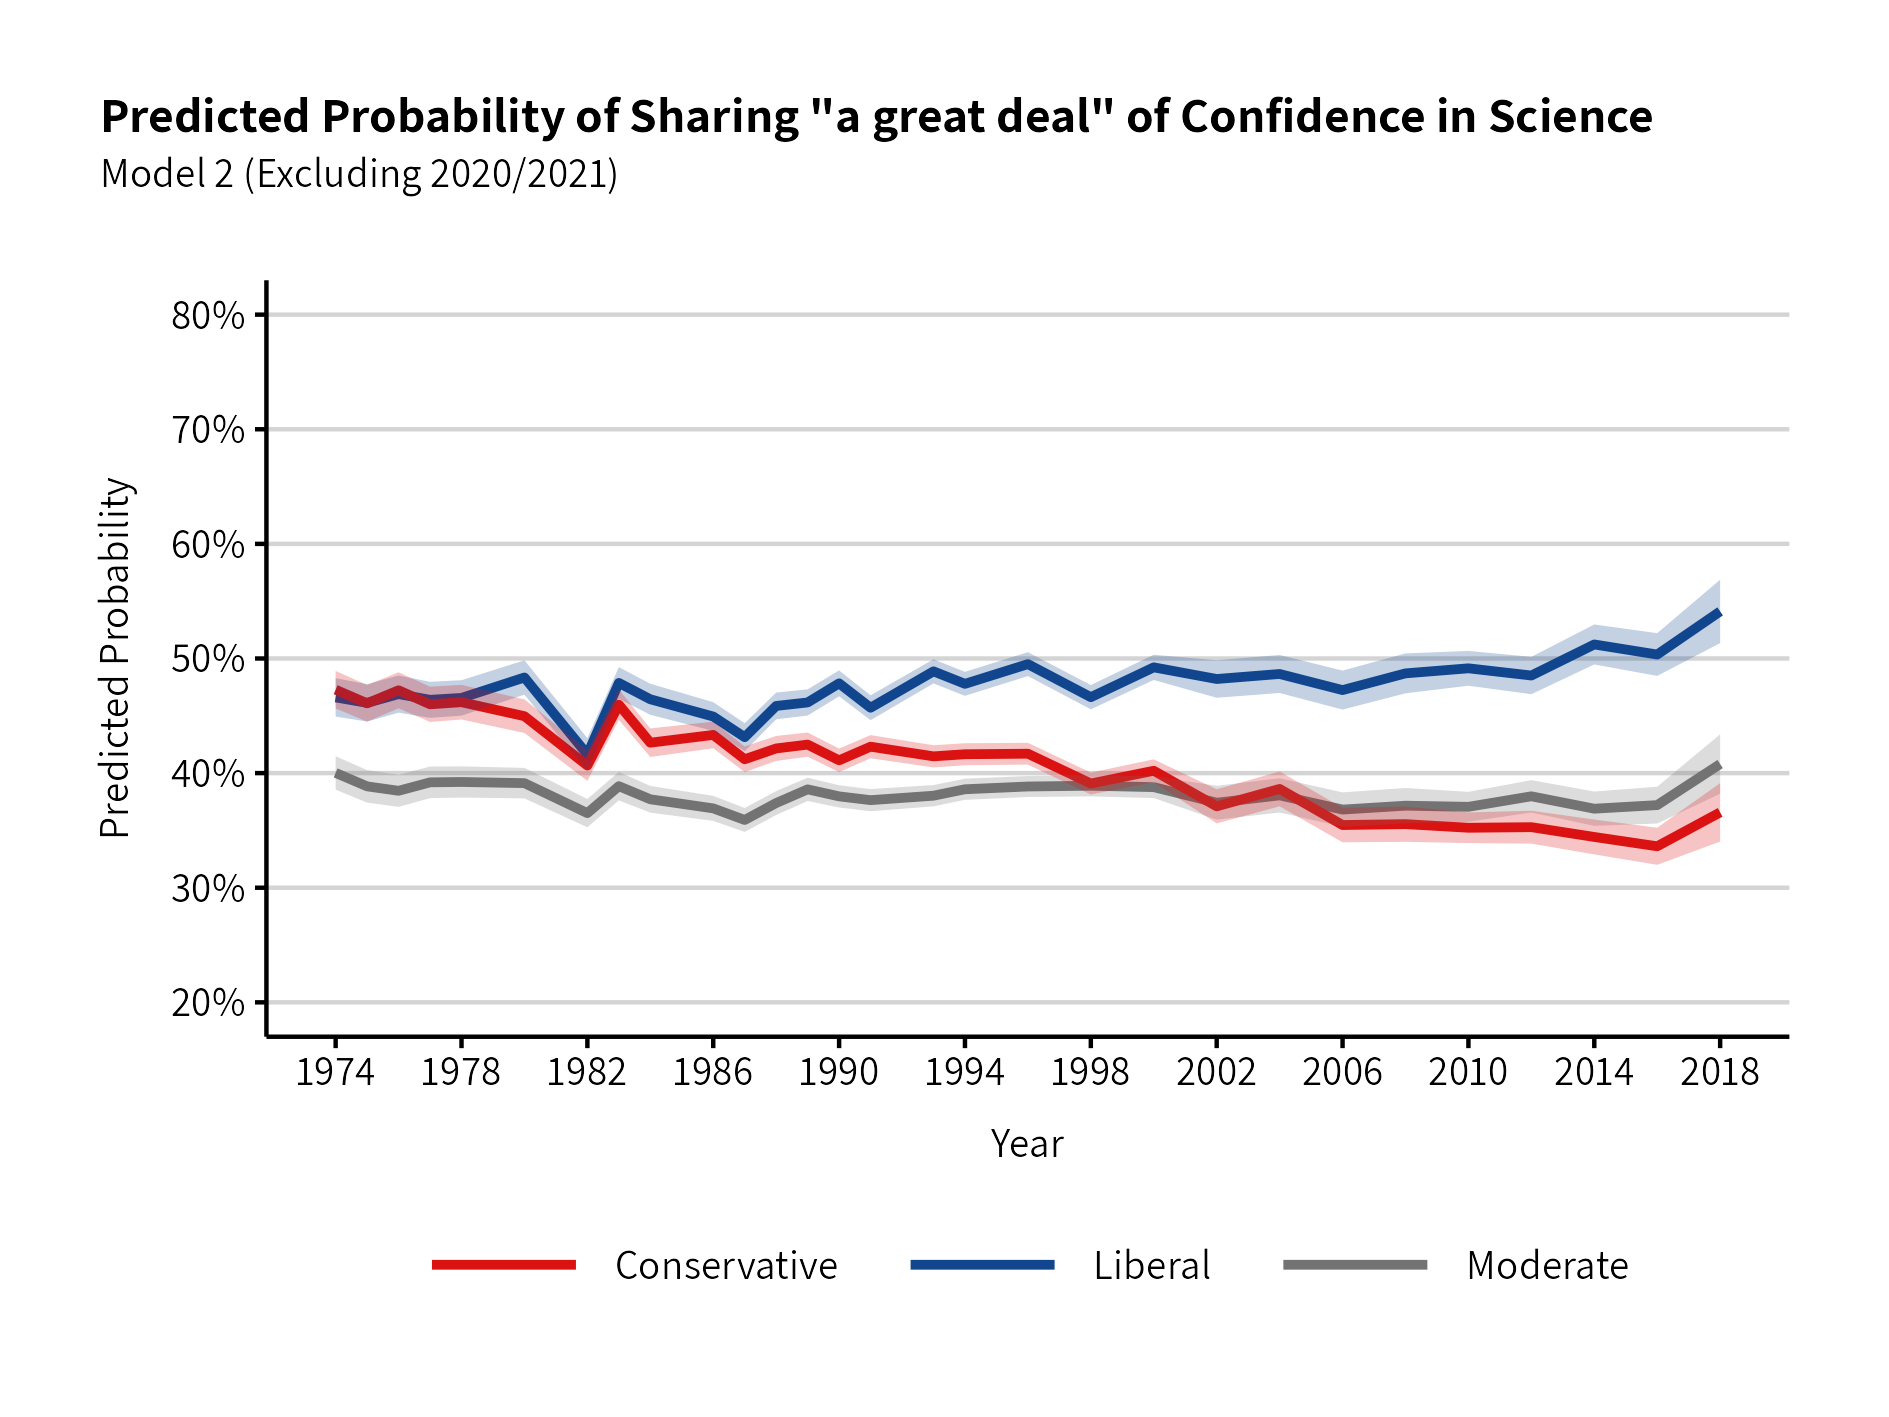
\includegraphics[width=0.8\paperwidth, keepaspectratio]{ {../figures/predict-polview-year-model-2} }
	}
\end{figure}
\end{frame}

\begin{frame}{Predicted Trust in Science, \textit{Excluding} 2021 (3)}
\begin{figure}
	\centerline{
		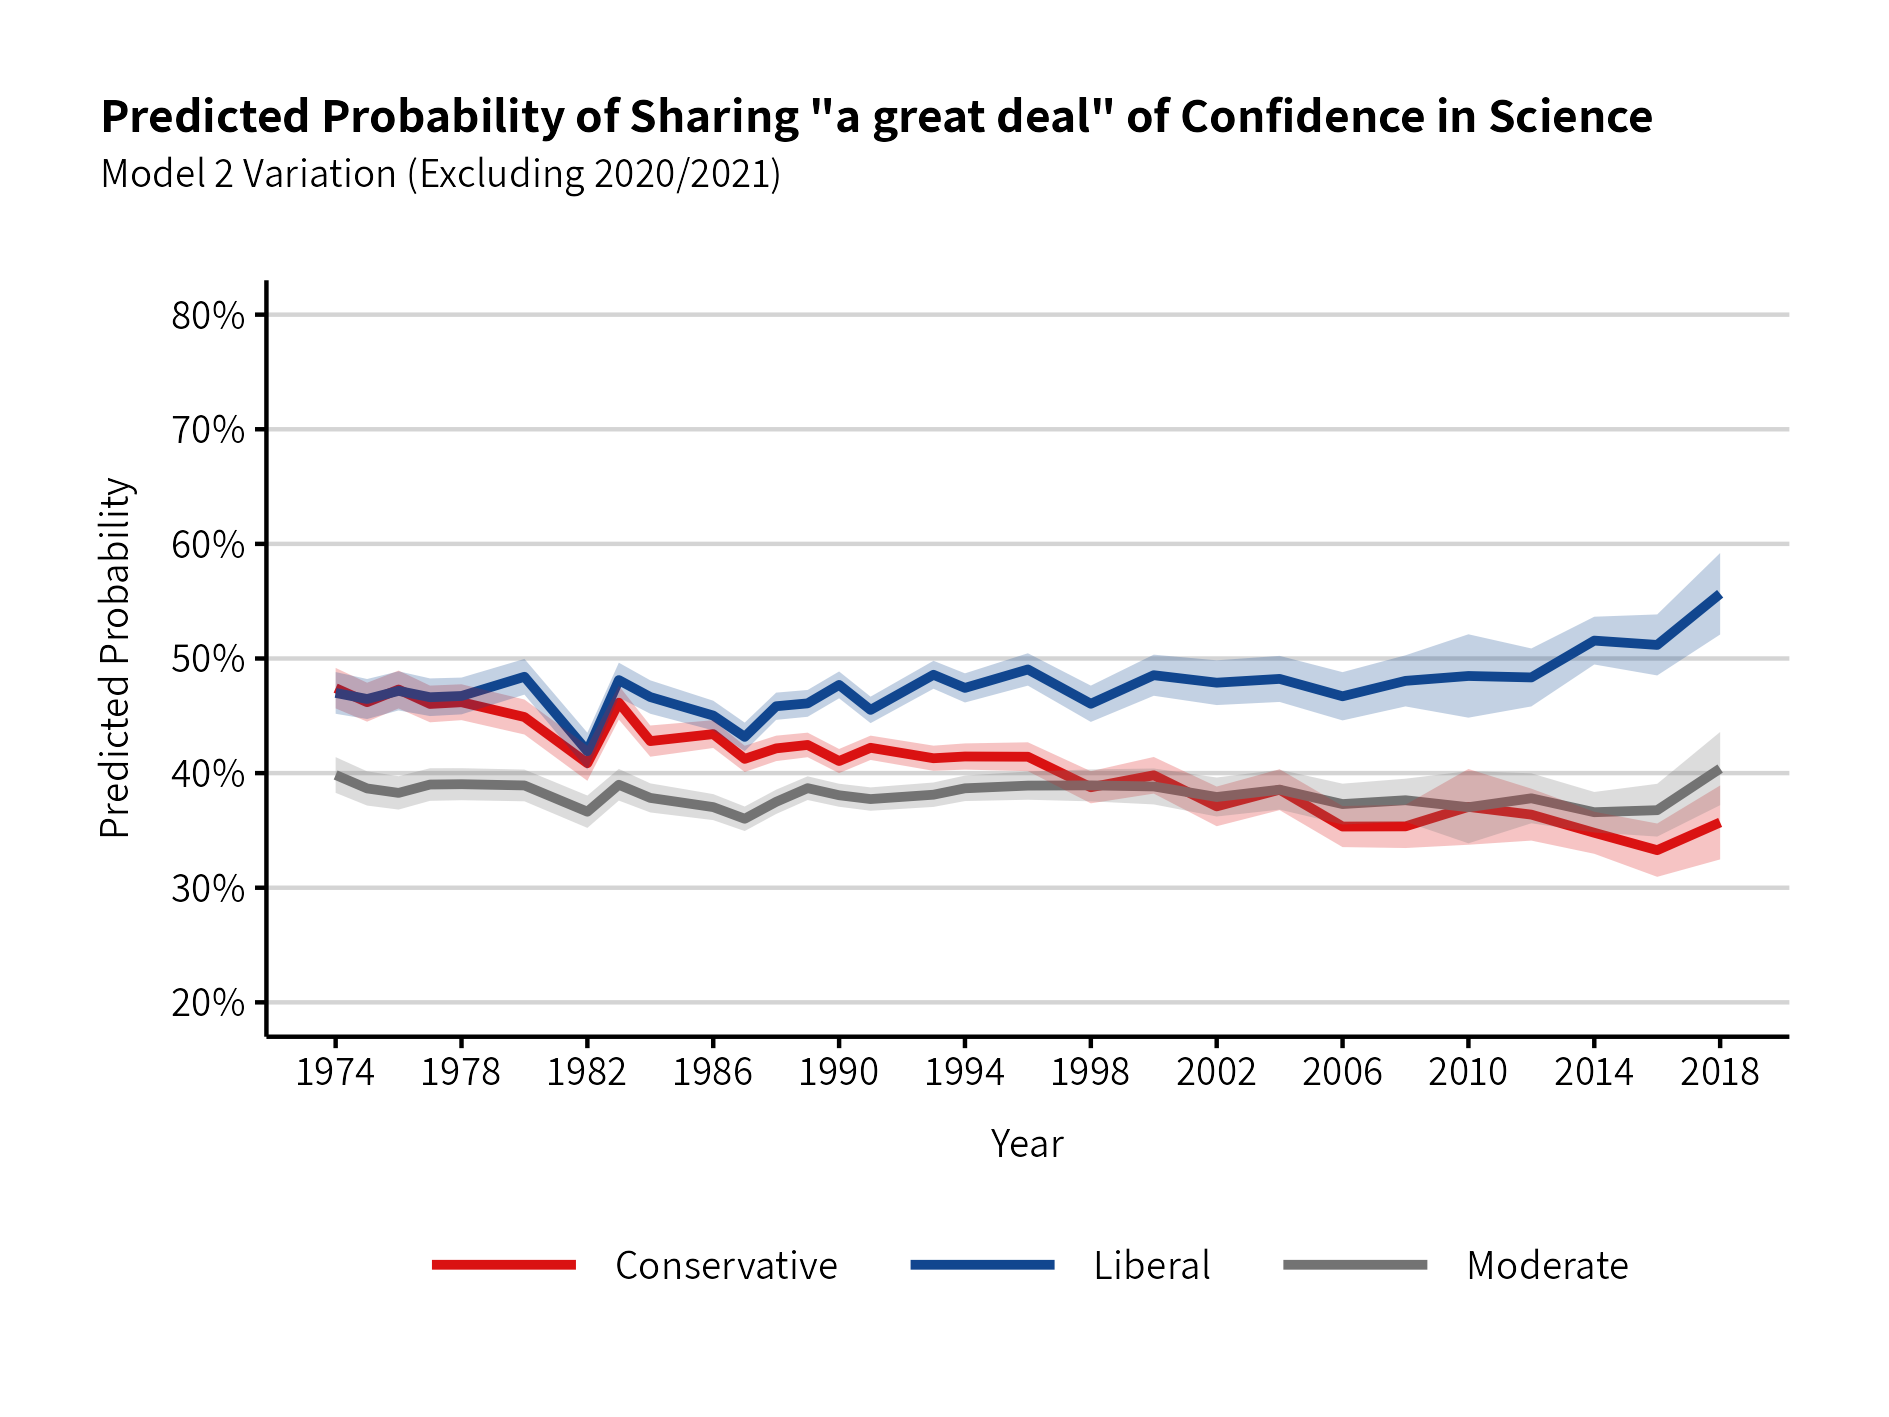
\includegraphics[width=0.8\paperwidth, keepaspectratio]{ {../figures/predict-polview-year-model-2-variation} }
	}
\end{figure}
\end{frame}

\begin{frame}{Predicted Trust in Science, \textit{Excluding} 2021 (4)}
\begin{figure}
	\centerline{
		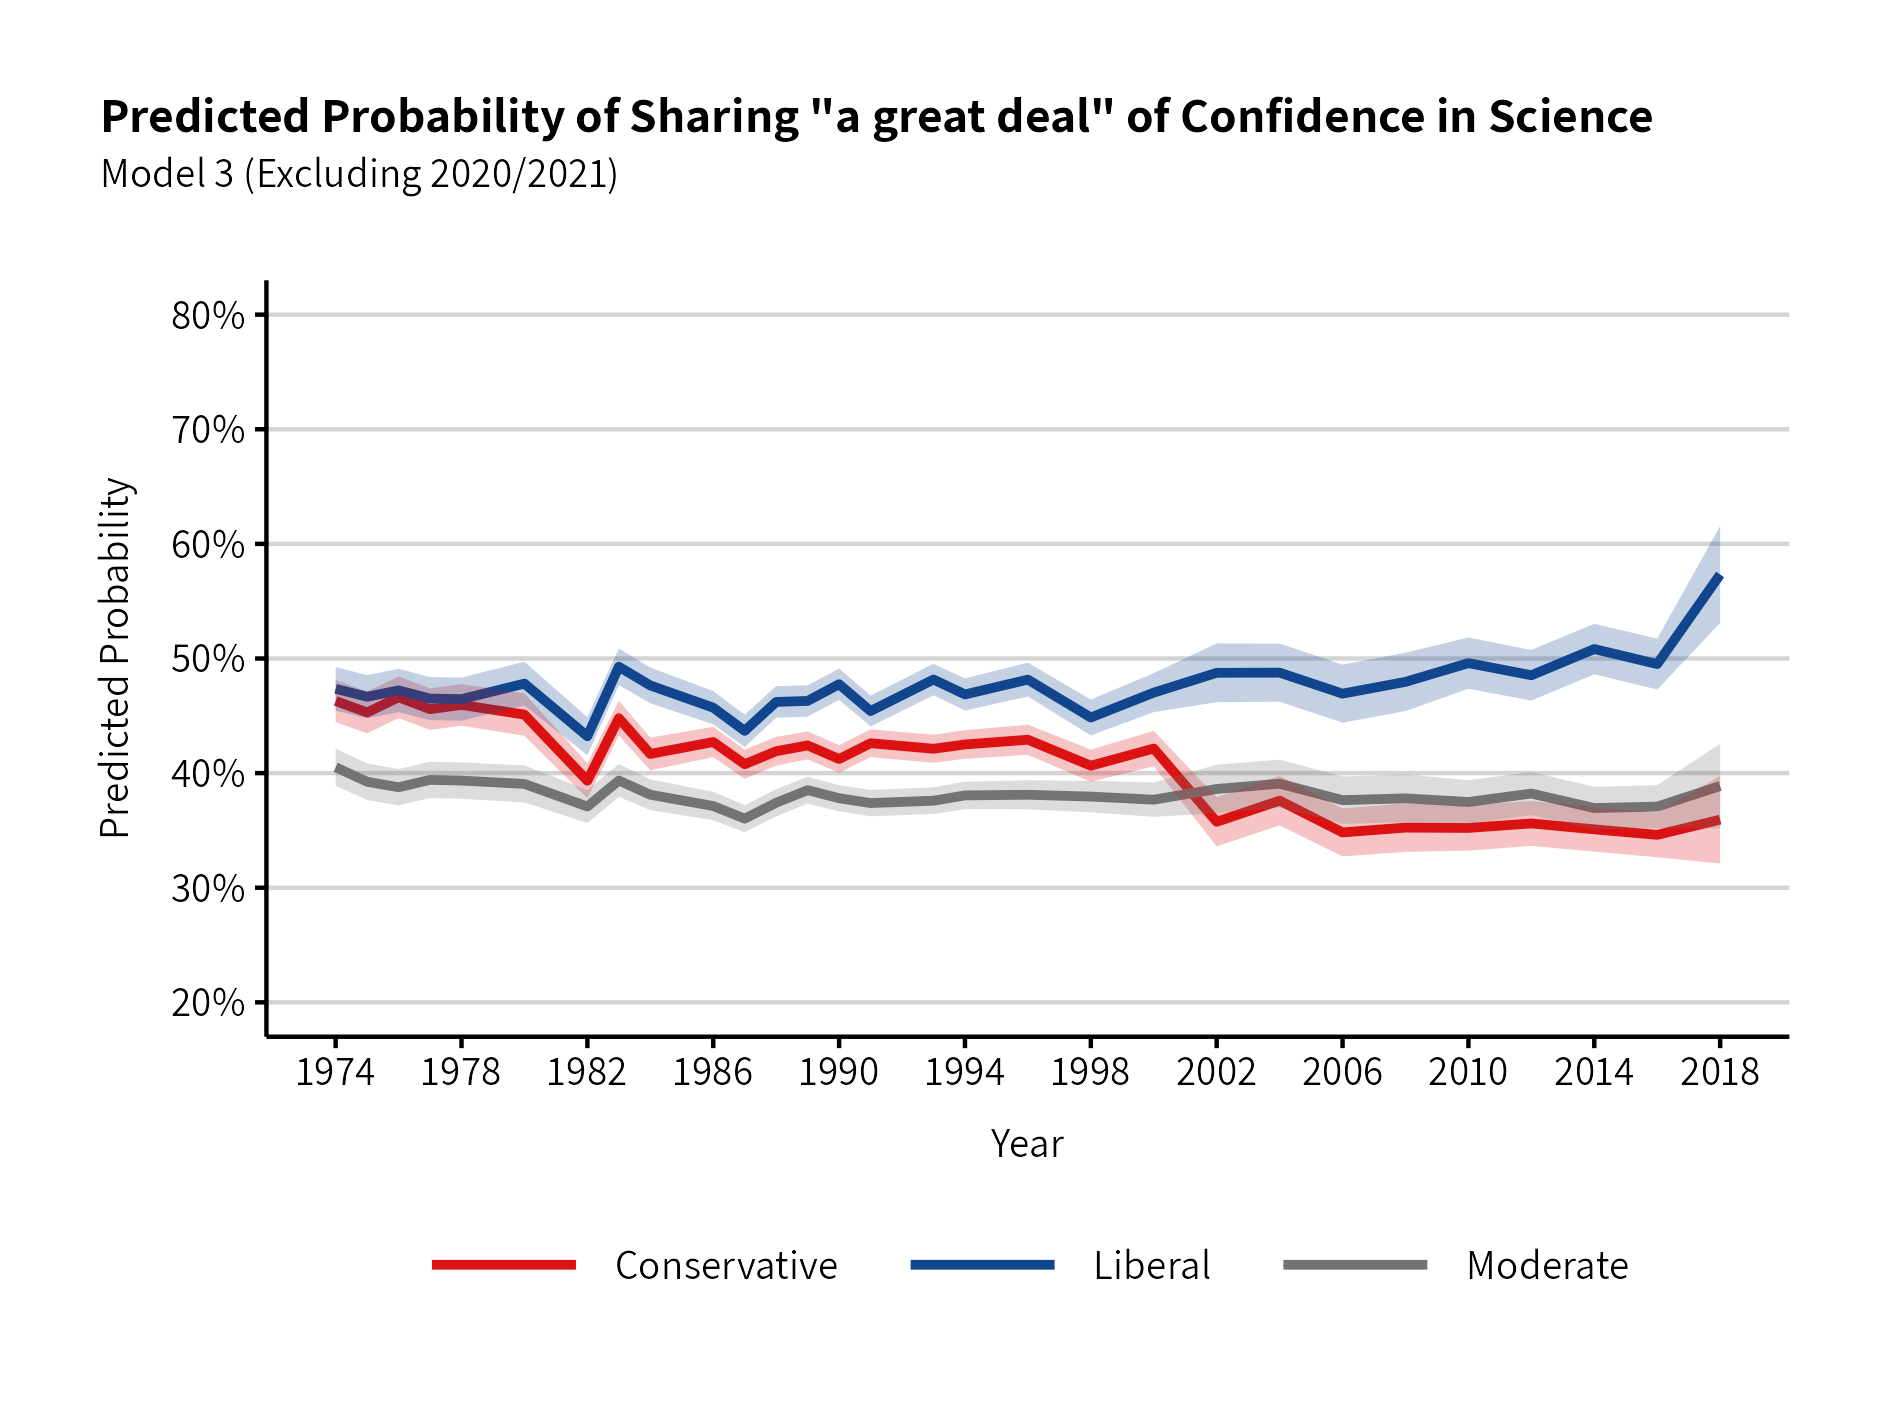
\includegraphics[width=0.8\paperwidth, keepaspectratio]{ {../figures/predict-polview-year-model-3} }
	}
\end{figure}
\end{frame}


\subsection{Predicted Trust in Science, \textit{Including} 2021}

\begin{frame}{Predicted Trust in Science, \textit{Including} 2021 (1)}
\begin{figure}
	\centerline{
		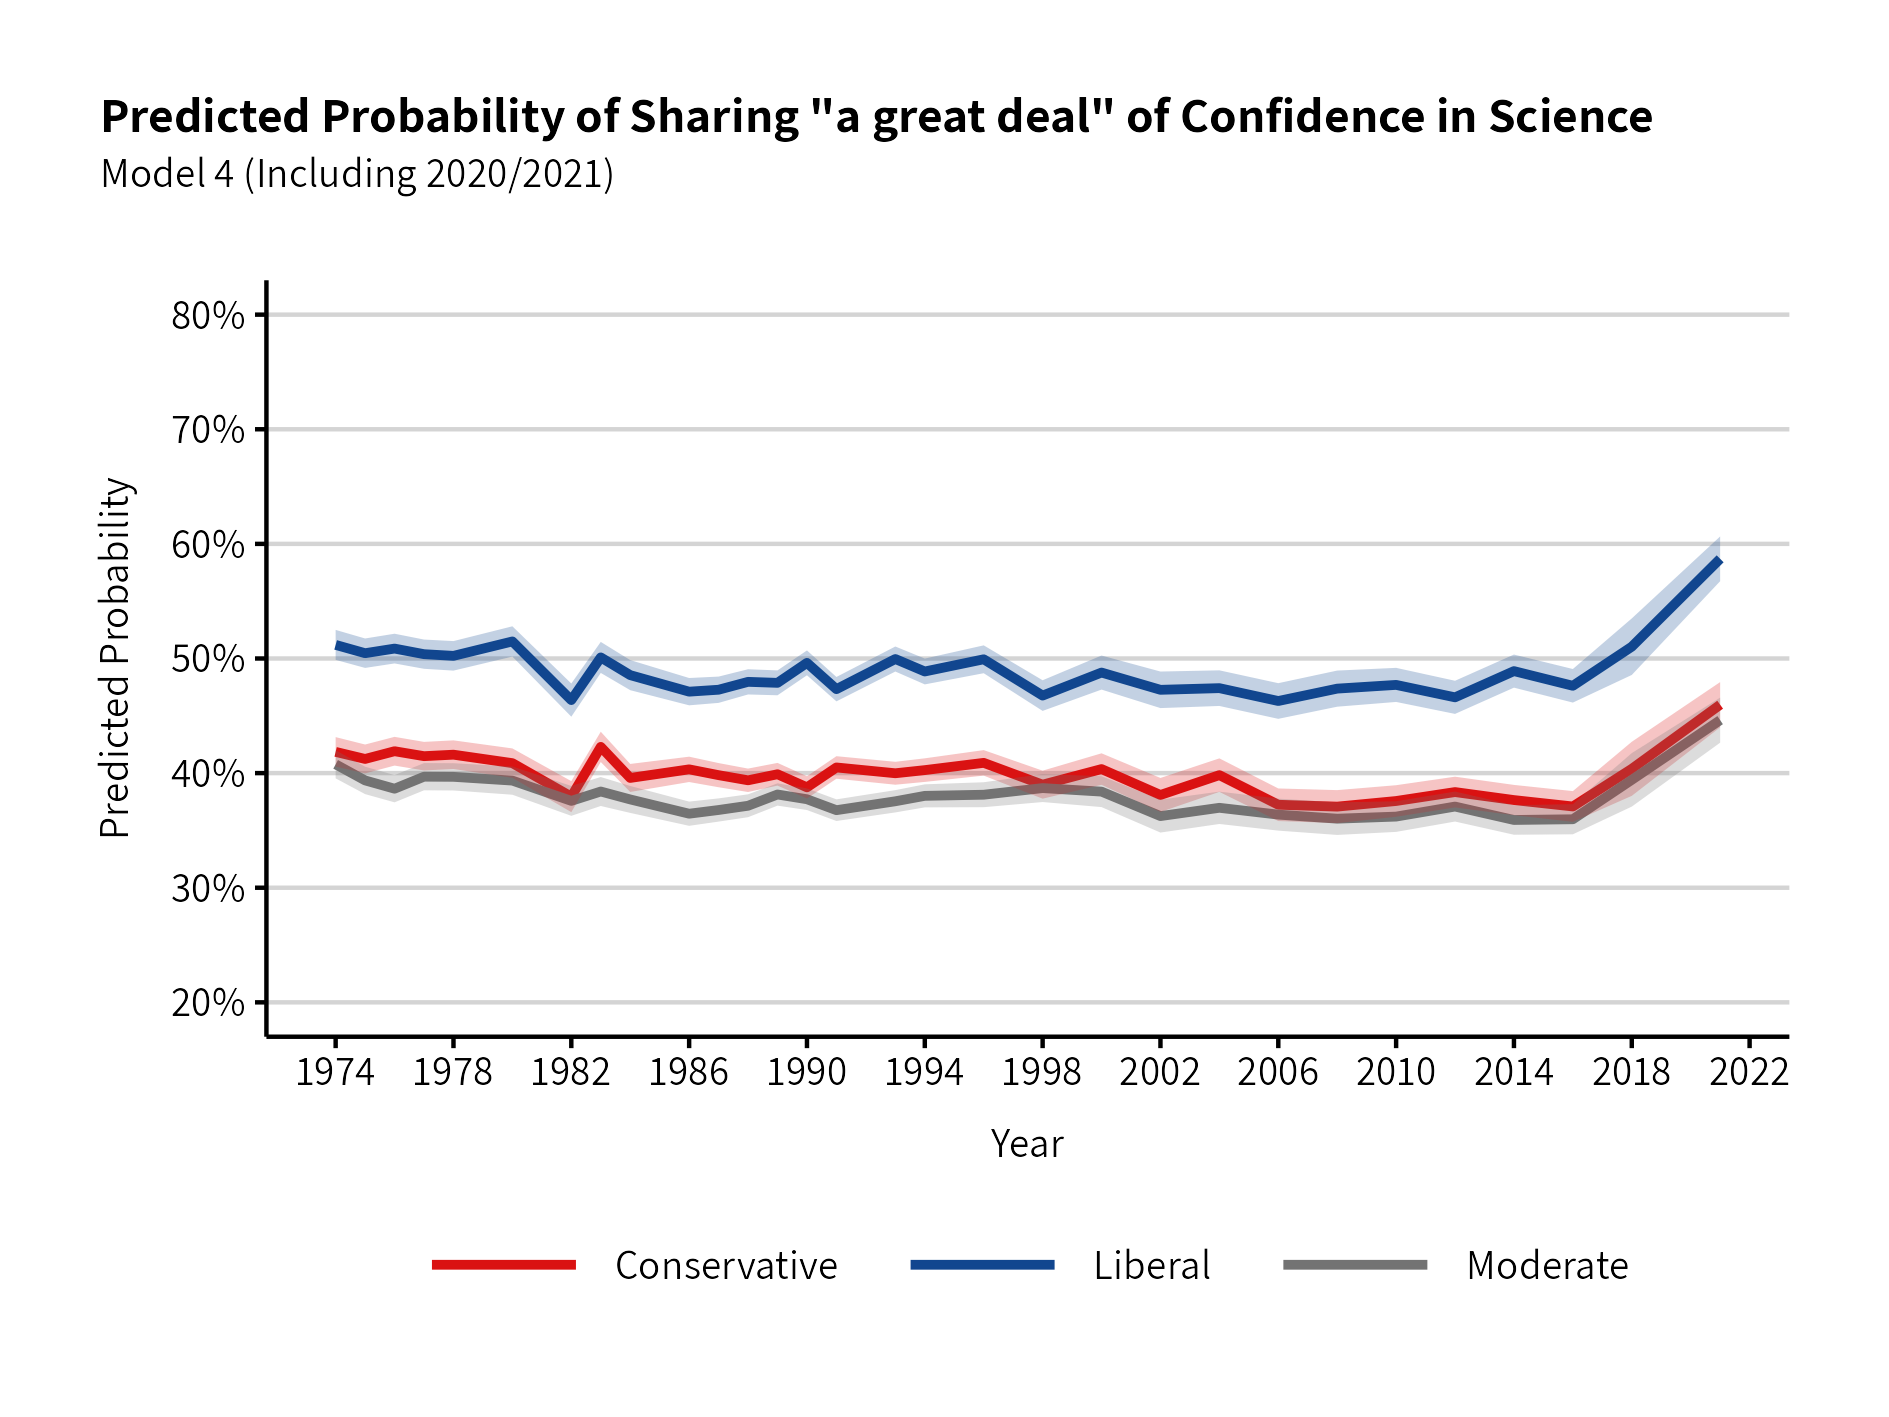
\includegraphics[width=0.8\paperwidth, keepaspectratio]{ {../figures/predict-polview-year-model-4} }
	}
\end{figure}
\end{frame}

\begin{frame}{Predicted Trust in Science, \textit{Including} 2021 (2)}
\begin{figure}
	\centerline{
		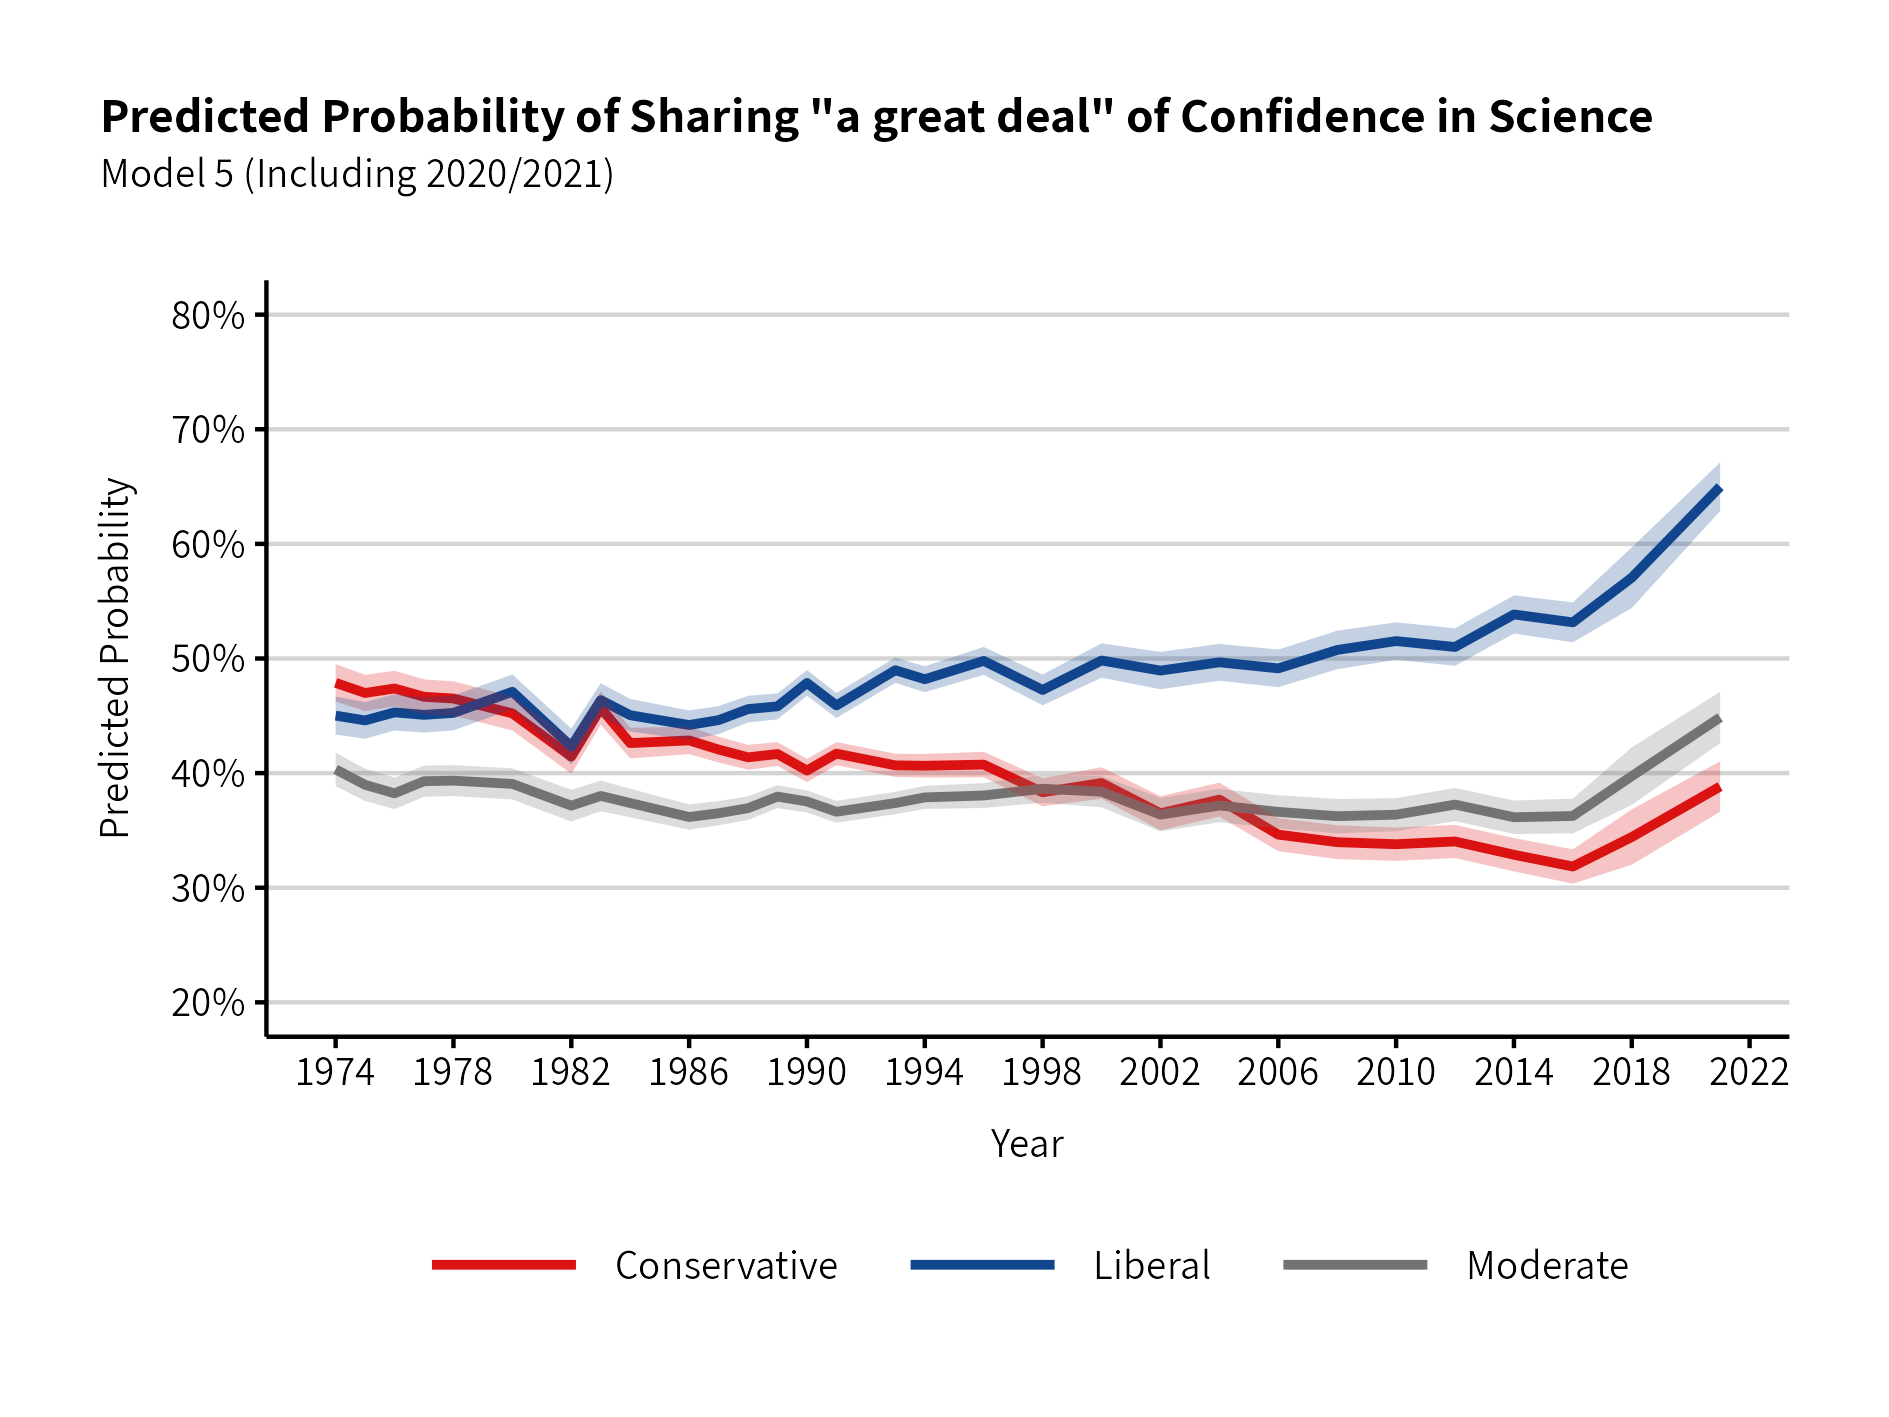
\includegraphics[width=0.8\paperwidth, keepaspectratio]{ {../figures/predict-polview-year-model-5} }
	}
\end{figure}
\end{frame}

\begin{frame}{Predicted Trust in Science, \textit{Including} 2021 (3)}
\begin{figure}
	\centerline{
		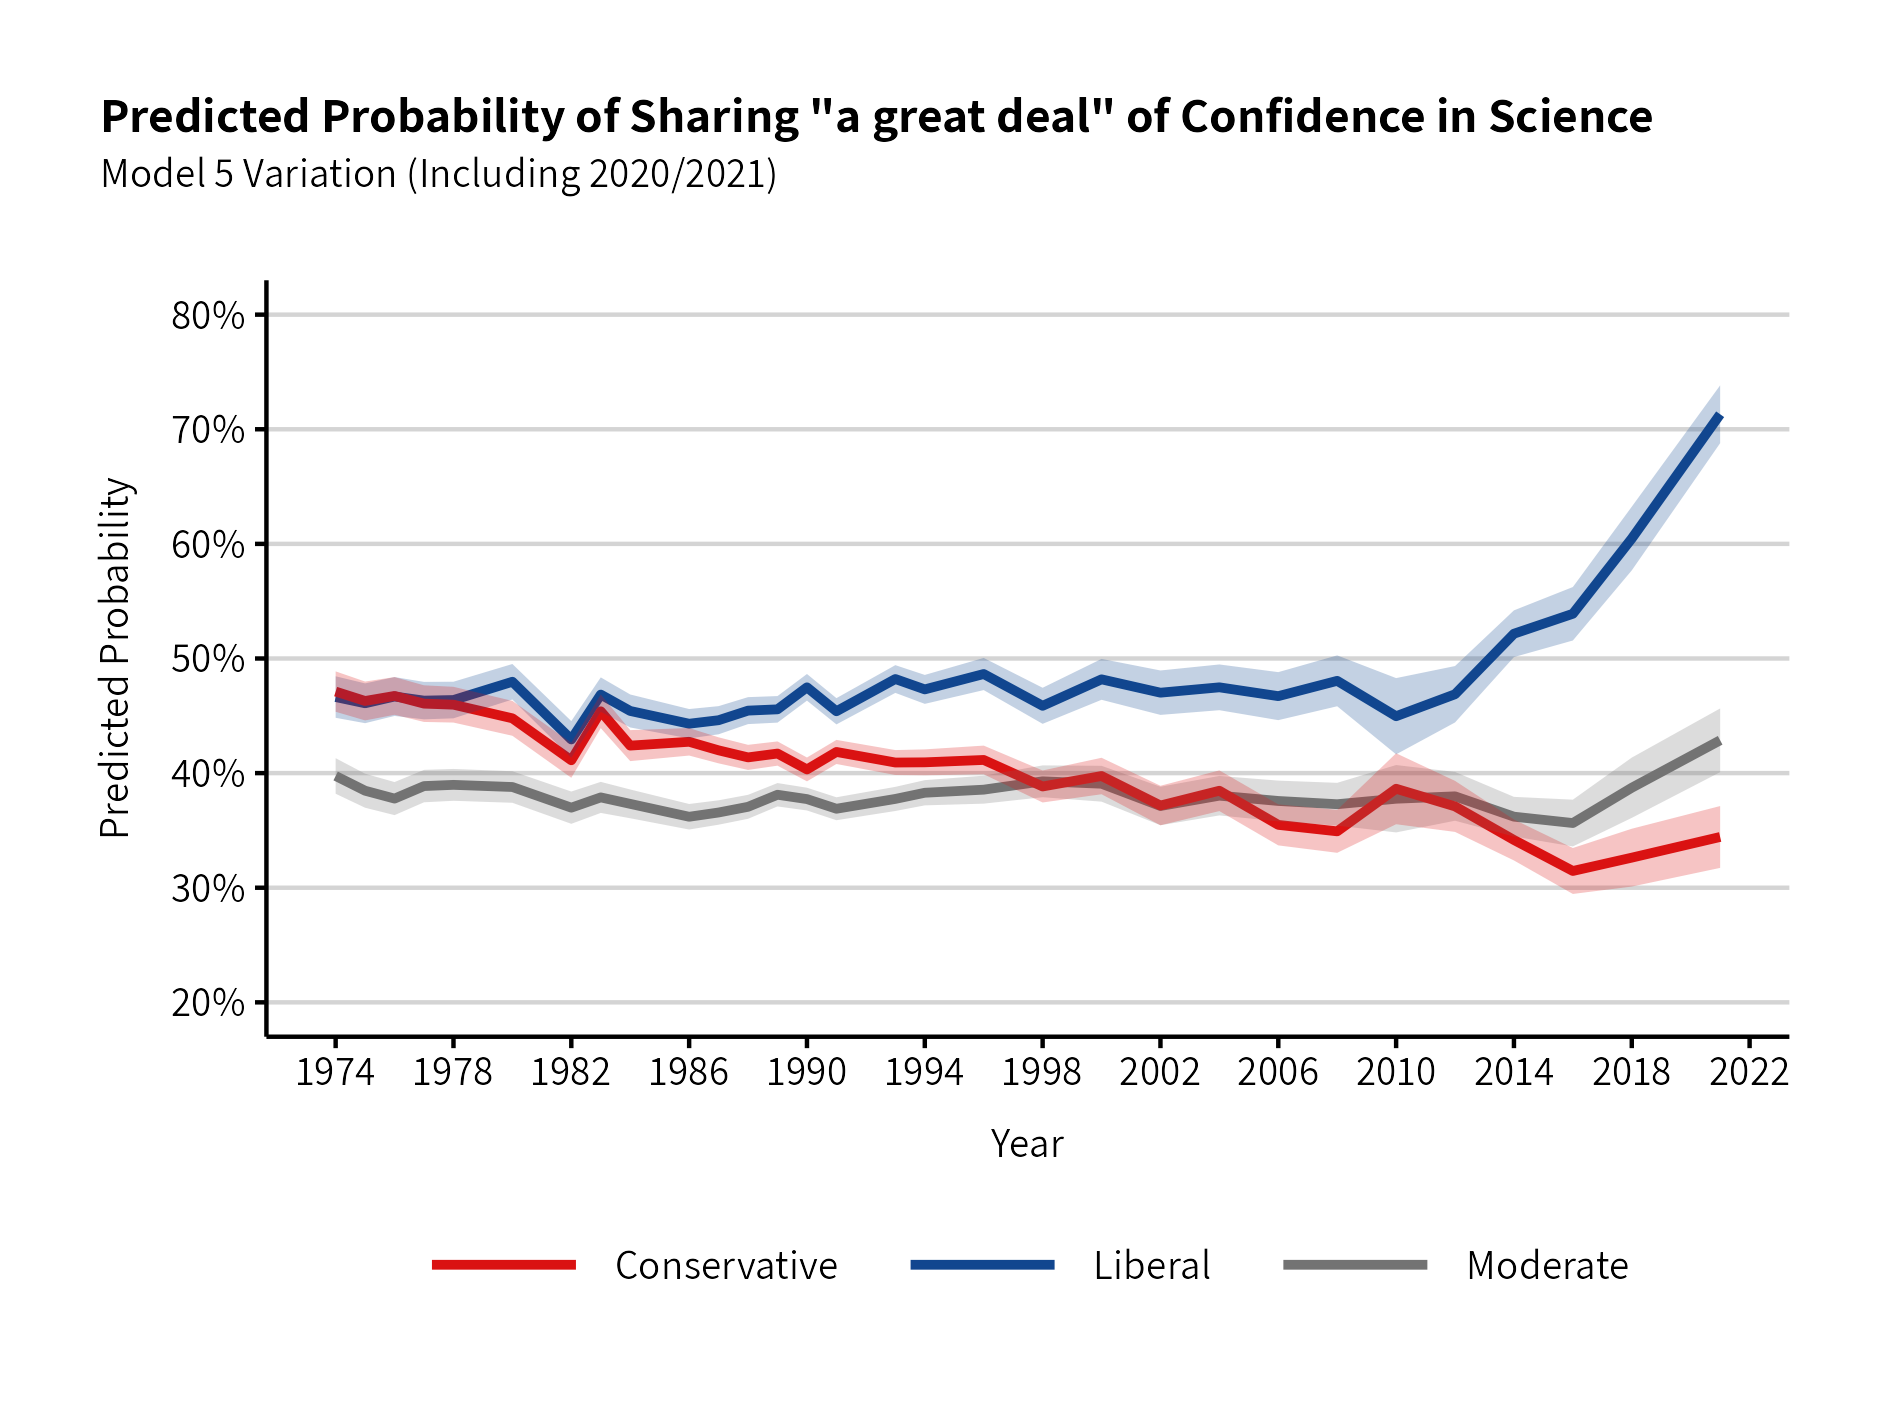
\includegraphics[width=0.8\paperwidth, keepaspectratio]{ {../figures/predict-polview-year-model-5-variation} }
	}
\end{figure}
\end{frame}

\begin{frame}{Predicted Trust in Science, \textit{Including} 2021 (4)}
\begin{figure}
	\centerline{
		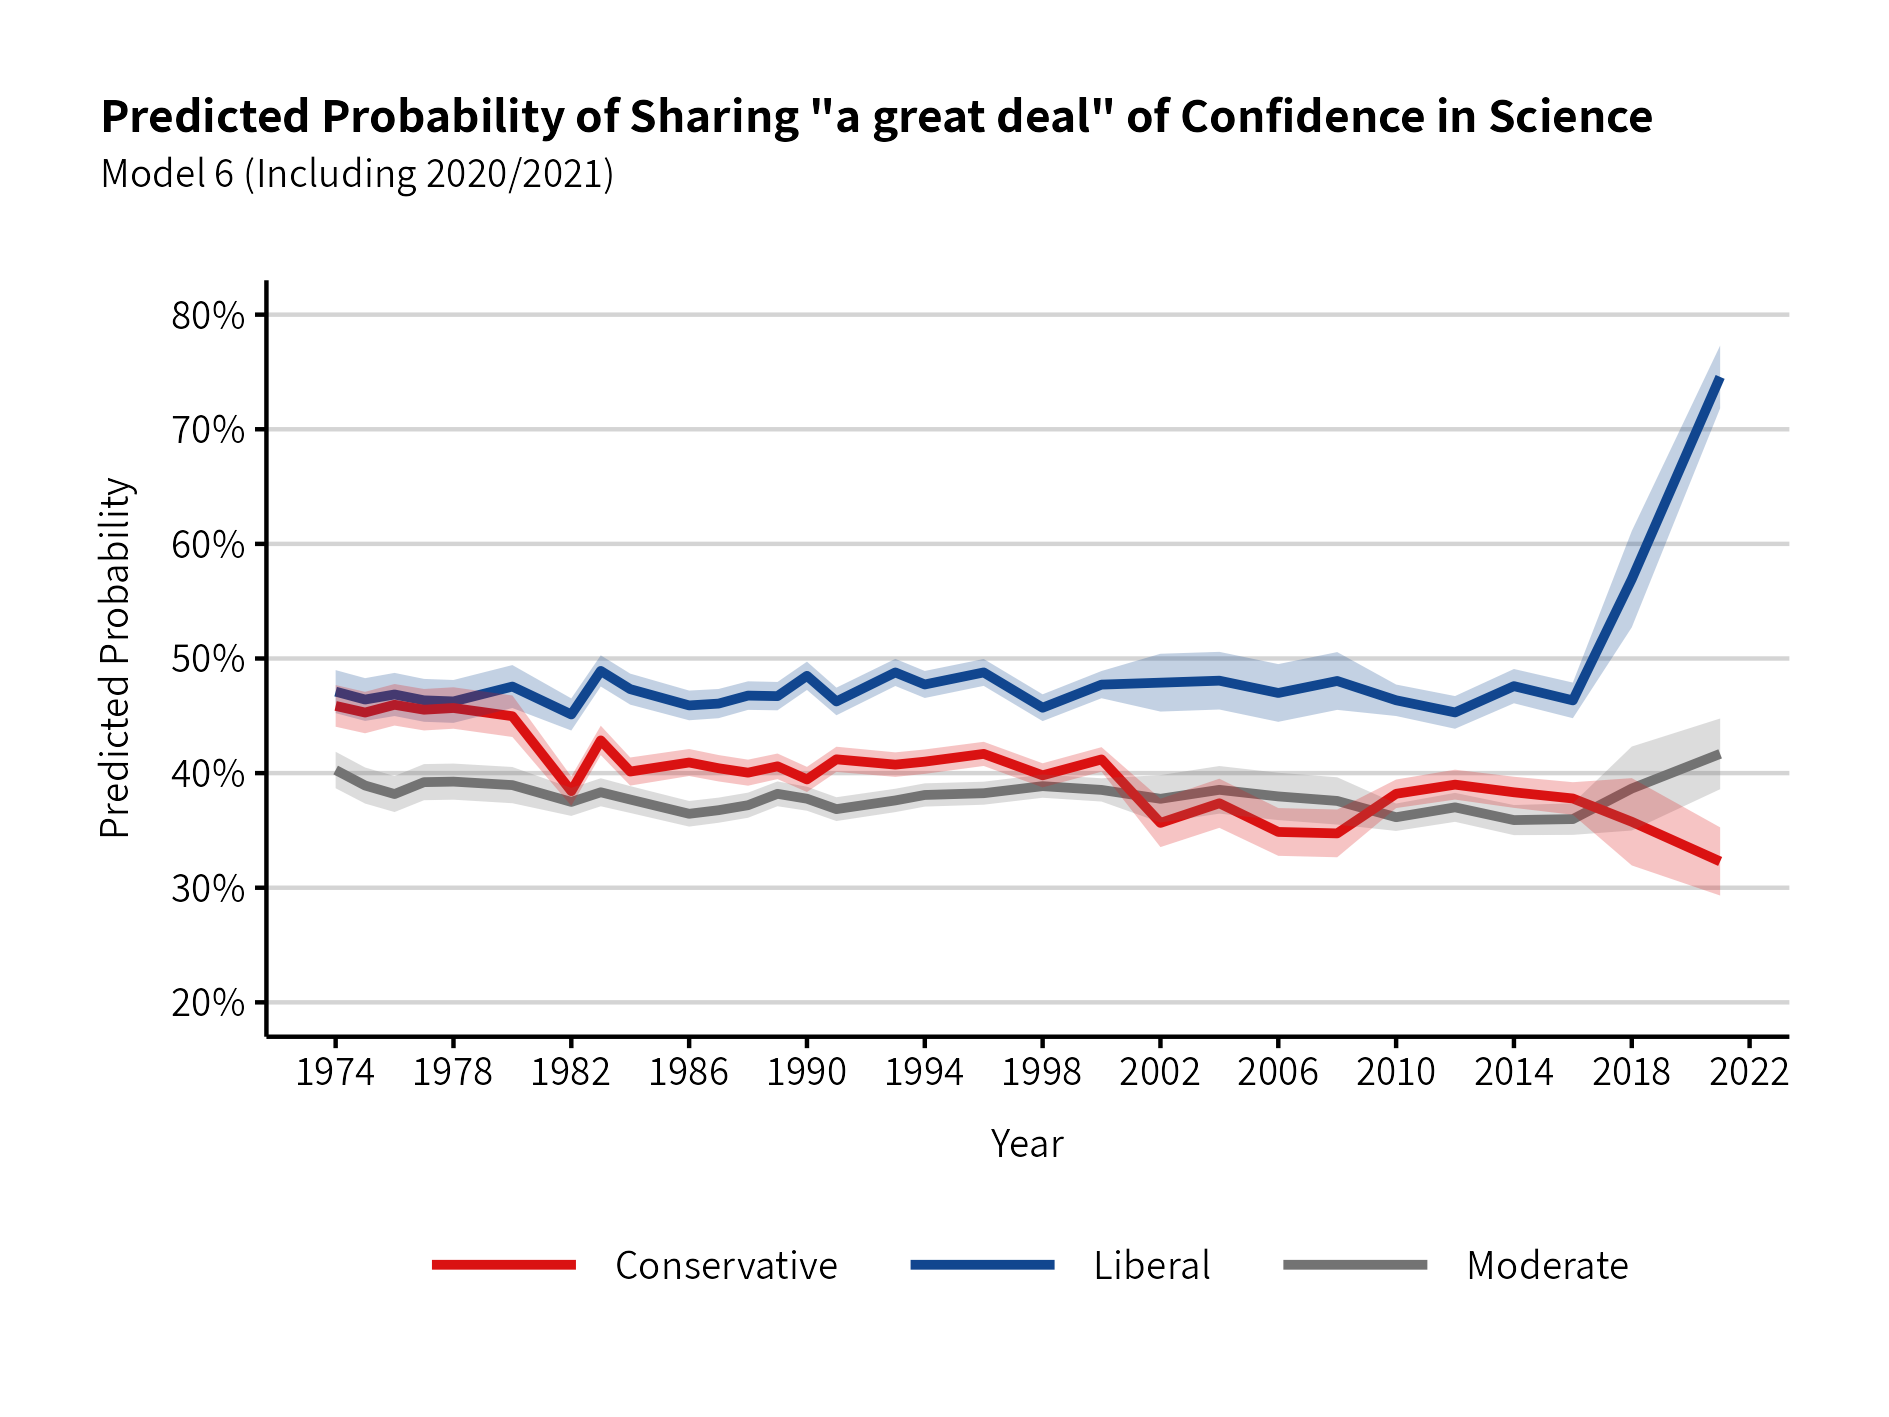
\includegraphics[width=0.8\paperwidth, keepaspectratio]{ {../figures/predict-polview-year-model-6} }
	}
\end{figure}
\end{frame}


% Disable the title page for the next section
\NextSectionWithoutTitlePage
\section{Appendix}

\begin{frame}{Appendix}
	Please find the data sets, scripts, and other supporting files and documents in the project's GitHub repository at \url{https://github.com/clemensheithecker/bachelor-thesis}.
\end{frame}


% Disable the title page for the next section
\NextSectionWithoutTitlePage
\section{References}

\begin{frame}[t]{References}
	\printbibliography[heading=none]
\end{frame}

\end{document}